\section{Multiple point clouds alignment}
\label{section:Registration}
When a scene is seen by several cameras, one needs to align the point of views in order to obtain a reconstruction of this scene. This problem is known as registration or stereo calibration. The goal is to find the relative positions and orientations of the separately acquired views in a global coordinate framework, such that the intersecting areas between them overlap perfectly.

The purpose of this section is to present the different methods of registration found in the literature. It proposes a different solution and compares it regarding the traditional ones.

\subsection{Theory}

Registration is the process of finding a spatial transformation that aligns two point sets or 3D point clouds. The goal is to find the relative position and orientation of the different acquired views in a global coordinate framework. The intersection between the different point cloud data views must overlap perfectly. This problem is often referred as pairwise registration.
The goal is to find a rigid body 4x4 transformation matrix (\ref{equation:rigid_transformation_matrix}) which is composed of a 3x3 rotation matrix \textbf{R} and a 3x1 translation vector \textbf{t}. \textit{Rigid body} means that the proportion of the 'body', e.g. the point cloud, are preserved. This transformation is applied to one of the point cloud (the source) in order to be perfectly aligned with the other point cloud (the target). Figure \ref{figure:transformation_matrix} illustrates the problem.

\begin{figure}[H]
    \centering
    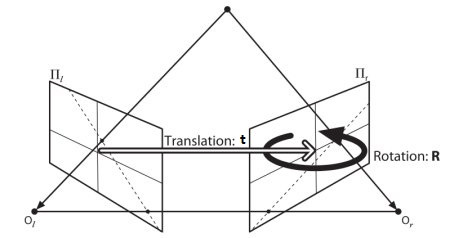
\includegraphics[width=0.65\textwidth]{images/registration/essential_matrix.jpg}
    \caption{Illustration of the registration problem. \textbf{R} and \textbf{t} have to be found to align two different views of the same scene. $O_l$ and $O_r$ are the camera centres. Source: \cite{noauthor_epipolar_nodate}}
    \label{figure:transformation_matrix}
\end{figure}

\begin{equation}
\label{equation:rigid_transformation_matrix}
\mathbf{M}=\left[\begin{array}{ll}
{\mathbf{R}} & {\mathbf{t}} \\
{\mathbf{0}^T} & {1}
\end{array}\right]
\end{equation}


The following matrices defines the rotation around the x,y and z-axis, explained in \cite{noauthor_rotation_2020}.

\begin{equation}
\mathbf{R}_{x}=\left[\begin{array}{ccc}
{1} & {0} & {0} \\
{0} & {\cos \theta_{x}} & {-\sin \theta_{x}} \\
{0} & {\sin \theta_{x}} & {\cos \theta_{x}}
\end{array}\right], \mathbf{R}_{y}=\left[\begin{array}{ccc}
{\cos \theta_{y}} & {0} & {\sin \theta_{y}} \\
{0} & {1} & {0} \\
{-\sin \theta_{y}} & {0} & {\cos \theta_{y}}
\end{array}\right], \mathbf{R}_{z}=\left[\begin{array}{ccc}
{\cos \theta_{z}} & {-\sin \theta_{z}} & {0} \\
{\sin \theta_{z}} & {\cos \theta_{z}} & {0} \\
{0} & {0} & {1}
\end{array}\right]
\end{equation}

\newpage
where:
\begin{itemize}
    \item $\theta_{x}$ is the rotation around the x-axis
    \item $\theta_{y}$ is the rotation around the y-axis
    \item $\theta_{z}$ is the rotation around the z-axis
\end{itemize}

The general rotation matrix can be obtained by multiplying these three rotation matrices.
% \begin{gather}
% \mathbf{R}=\mathbf{R}_{z} \mathbf{R}_{y}\mathbf{R}_{x}\\
% =\left[\begin{array}{ccc}
% {\cos \theta_{y} \cos \theta_{z}} & {-\cos \theta_{y} \sin \theta_{z}} & {\sin \theta_{y}} \\
% {\cos \theta_{x} \sin \theta_{z}+\cos \theta_{z} \sin \theta_{x} \sin \theta_{y}} & {\cos \theta_{x} \cos \theta_{z}-\sin \theta_{x} \sin \theta_{y} \sin \theta_{z}} & {-\cos \theta_{y} \sin \theta_{x}} \\
% {\sin \theta_{x} \sin \theta_{z}} & {-\cos \theta_{x} \cos \theta_{z} \sin \theta_{y}} & {\cos \theta_{z} \sin \theta_{x}+\cos \theta_{x} \sin \theta_{y} \sin \theta_{z}} & {\cos \theta_{x} \cos \theta_{y}}
% \end{array}\right]
% \end{gather}

\begin{gather}
\mathbf{R}=\mathbf{R}_{z} \mathbf{R}_{y}\mathbf{R}_{x}\\
=\left[\begin{array}{ccc}\cos \theta_{z} \cos \theta_{y} & \cos \theta_{z} \sin \theta_{y} \sin \theta_{x}-\sin \theta_{z} \cos \theta_{x} & \cos \theta_{z} \sin \theta_{y} \cos \theta_{x}+\sin \theta_{z} \sin \theta_{x} \\ \sin \theta_{z} \cos \theta_{y} & \sin \theta_{z} \sin \theta_{y} \sin \theta_{x}+\cos \theta_{z} \cos \theta_{x} & \sin \theta_{z} \sin \theta_{y} \cos \theta_{x}-\cos \theta_{z} \sin \theta_{x} \\ -\sin \theta_{y} & \cos \theta_{y} \sin \theta_{x} & \cos \theta_{y} \cos \theta_{x}\end{array}\right]
\end{gather}

The translation vector is defined as follow:

\begin{equation}
\mathbf{t}=\left[\begin{array}{ll}
t_x \\
t_y \\
t_z
\end{array}\right]
\end{equation}

where:
\begin{itemize}
    \item $t_x$ is the translation along the x-axis
    \item $t_y$ is the translation along the y-axis
    \item $t_z$ is the translation along the z-axis
\end{itemize}
\subsection{Previous work and usual approaches}
\label{section:registration_previous_work}
Several methods exist to estimate the transformation matrix. Iterative closest point (ICP) and other registration methods need an approximate initial guess to avoid converging in wrong local minima. They are applied directly in the 3D space. Other methods compute the 3D pose estimation of an object relative to the first and to the second camera from 2D images. Then they compute a transformation matrix to go from one view into the other one. This section develops some of the relevant approaches found in the literature.

% Other methods use 2D images. The strategy consists in:

% \begin{enumerate}
%     \item Finding keypoints/objects in the two images
%     \item Matching corresponding keypoints/objects in the two images
%     \item Finding
% \end{enumerate}

\subsubsection{Iterative closest point registration}
\label{section:Iterative closest point registration}

The ICP algorithm proposed by \cite{besl_method_1992} and \cite{chen_object_1992} is commonly used for alignment of 3D objects or scenes when an initial estimate of the relative pose is known. This algorithm is applied directly in the 3D space after the creation of the point clouds acquired from different views. The goal of ICP is to minimise the distance between two point sets.

$\mathbf{P}=\left\{p_{1} \ldots p_{N_{P}}\right\}$ is the target point cloud and $\mathbf{Q}=\left\{q_{1} \ldots q_{N_{Q}}\right\}$ is called the source point cloud.
 
 Different variants of ICP exist but they all iterate over the following steps in general:

\begin{enumerate}
    \item Select a subset of data from the two point clouds, $\mathbf{P}^{\prime}$ and $\mathbf{Q}^{\prime}$
    \item Find correspondences set $\mathcal{K} = \{(\mathbf{p}, \mathbf{q})\}$ from $\mathbf{P}^{\prime}$ and $\mathbf{Q}^{\prime}$
    \item Give an initial starting guess of the rigid body transformation and estimate the best $\mathbf{M}=\left[\begin{array}{ll}{\mathbf{R}} & {\mathbf{t}} \\ {\mathbf{0}^{T}} & {1}\end{array}\right]$ mapping $\mathbf{Q}^{\prime}$ onto $\mathbf{P}^{\prime}$
    \item Use the found $\mathbf{M}$ to transform $\mathbf{Q}^{\prime}$
    \item Update $\mathbf{M}$ by minimising an objective function $E(\mathbf{M})$ defined over the correspondence set $\mathcal{K}$
\end{enumerate}


\subsubsubsection{Point-to-point ICP}

The point-to-point ICP algorithm described in \cite{besl_method_1992} uses this objective function:

\begin{equation}
\label{equation:point-to-point}
E(\mathbf{M})=\sum_{(\mathbf{p}, \mathbf{q}) \in \mathcal{K}}\|\mathbf{p}-\mathbf{M} \mathbf{q}\|^{2}
\end{equation}

The purpose is to minimise the euclidean distance between the points of the two subsets $\mathbf{P}^{\prime}$ and $\mathbf{Q}^{\prime}$.


\subsubsubsection{Point-to-plane ICP}

The point-to-plane ICP algorithm described in \cite{chen_object_1992} uses this objective function:

\begin{equation}
\label{equation:point-to-plane}
E(\mathbf{M})=\sum_{(\mathbf{p}, \mathbf{q}) \in \mathcal{K}}\left((\mathbf{p}-\mathbf{M} \mathbf{q}) \cdot \mathbf{n}_{\mathbf{p}}\right)^{2}
\end{equation}

where $\mathbf{n}_{\mathbf{p}}$ is the normal of point $\mathbf{p}$.

\subsubsection{Coloured point cloud registration}
\label{section:Coloured point cloud registration}

\cite{park_colored_2017} proposes a variation of the ICP algorithm by adding the colour information to help finding a better transformation matrix $\mathbf{M}$. The objective function is the following:

\begin{equation}
\label{equation:coloured-ICP}
E(\mathbf{M})=(1-\delta) E_{C}(\mathbf{M})+\delta E_{G}(\mathbf{M})
\end{equation}

Where $\delta \in[0,1]$ is a weight parameter that has been determined empirically. $E_{C}$ is the colour term and $E_{G}$ is the geometric term. This geometric term $E_{G}$ is the same as the point-to-plane ICP objective, see equation (\ref{equation:point-to-plane}). The $E_{C}$ colour term is defined as follow:

\begin{equation}
E_{C}(\mathbf{M})=\sum_{(\mathbf{p}, \mathbf{q}) \in \mathcal{K}}\left(C_{\mathbf{p}}(\mathbf{f}(\mathbf{M} \mathbf{q}))-C(\mathbf{q})\right)^{2}
\end{equation}

where:

\begin{itemize}
    \item $C(\mathbf{q})$ is the colour of point $\mathbf{q}$
    \item $C_{\mathbf{p}}(\cdot)$ is is a precomputed function continuously defined on the tangent plane of $\mathbf{p}$
    \item $\mathbf{f}(\cdot)$ is a function that projects a 3D point to the tangent plane.
\end{itemize}

This colour term measures the difference between the colour of point $\mathbf{q}$. i.e. $C(\mathbf{q})$, and the colour of its projection on the tangent plane of $\mathbf{p}$. $C_{\mathrm{p}}(\cdot)$

\subsubsection{Global registration}
\label{section:Global registration}

\nameref{section:Iterative closest point registration} and \nameref{section:Coloured point cloud registration} rely on an estimation of the transformation matrix. They are known as local registration methods. Other registration methods that don't rely on a rough estimation of the alignment are known as global registration. They usually produce less good alignment results than the local one and are often used as initialisation for the local methods. \cite{noauthor_global_nodate} and \cite{gelfand_robust_nodate} present global registration algorithms. They are based on robust feature identification and correspondence search using geometric descriptors. The workflow of \cite{noauthor_global_nodate} is the following:

\begin{enumerate}
    \item \textbf{Extract geometric feature}. The point clouds are downsampled and their normals are estimated. Fast Point Feature Histogram (FPFH) are computed for each point. The FPFH feature is a 33-dimensional vector that describes the local geometric property of a point. \cite{rusu_fast_2009} explains FPFH for 3D registration in detail.
    
    \item \textbf{RANSAC}. Random points are picked from the source point cloud at each iteration. A nearest neighbour query is performed in the 33-dimensional FPFH feature space in the target point cloud. This query returns points with similar local geometric structures. Then pruning is performed to quickly reject false matches. The points that passed the pruning step are therefore used to compute the transformation matrix. It is then validated on the entire point cloud. This process stops after the RANSAC convergence criteria are reached.
    
    \item \textbf{Local refinement}. As the transformation matrix is calculated on down-sampled point clouds, the result is not tight. Point-to-plane ICP is used to refine the alignment. The other ICP methods could also be used.
\end{enumerate}


\subsubsection{Stereo calibration}

Stereo calibration is the process of computing the geometrical relationship between two cameras. This relationship is defined by the intrinsic and extrinsic parameters. Corresponding points have to be found in both perspectives to estimate this relationship. The method minimises the total re-projection error for all the points in all the available views from both cameras. A checker board is used in \cite{rathnayaka_efficient_2017} to determine these corresponding points. Other easily detectable patterns as ChArUco board, chessboard, circle grid or random pattern calibration object could be used instead, see figure \ref{figure:pattern}. \cite{liu_stereo_2009} uses Scale-Invariant Feature Transform (SIFT) to determine these corresponding points. SIFT is a method used to find certain features point in 2D images. It doesn't need to put a specific pattern in the scene which is an advantage. However, according to \cite{liu_stereo_2009}, wrong matching points are found sometimes. This affects the quality of the transformation matrix.

\begin{figure}[H]
\centering
  \begin{subfigure}[b]{0.24 \textwidth}
    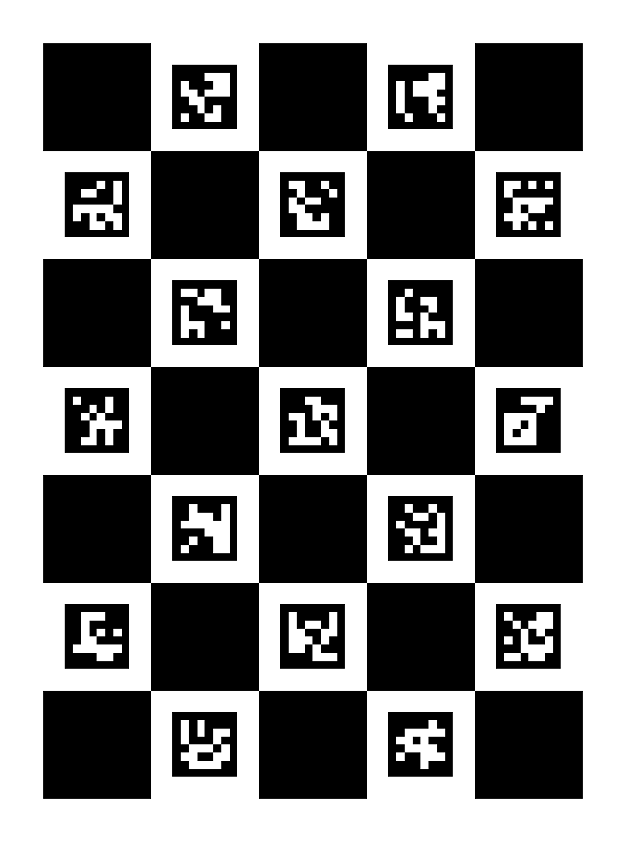
\includegraphics[width=\textwidth]{images/registration/charucoboard.png}
    \caption{Chessboard pattern}
    \label{figure:charucoboard}
  \end{subfigure}
  \hfill
  \begin{subfigure}[b]{0.24 \textwidth}
    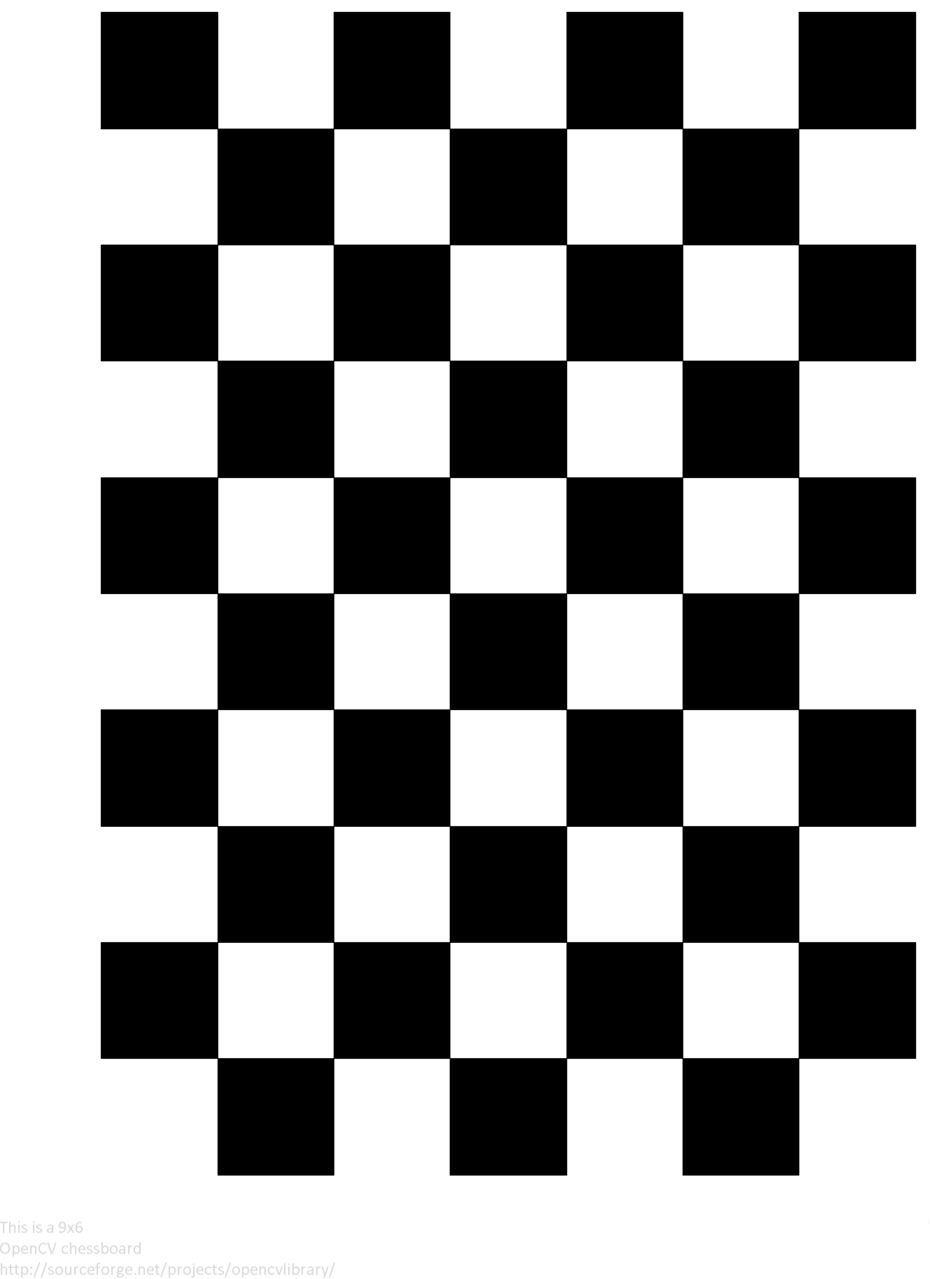
\includegraphics[width=\textwidth]{images/registration/chessboard.jpg}
    \caption{Chessboard pattern}
    \label{figure:chessboard}
  \end{subfigure}
  \hfill
  \begin{subfigure}[b]{0.24\textwidth}
    
\includegraphics[width=\textwidth]{images/registration/circle_pattern.png}
    \caption{Circle grid pattern}
    \label{figure:circle_pattern}
  \end{subfigure}
  \hfill
  \begin{subfigure}[b]{0.24\textwidth}
    
\includegraphics[width=\textwidth]{images/registration/random_pattern.jpg}
    \caption{Random pattern}
    \label{figure:random_pattern}
  \end{subfigure}
  \caption{Easily detectable patterns provided by OpenCV \cite{noauthor_opencv_nodate}}
  \label{figure:pattern}
\end{figure}


\subsubsection{Deep Learning}

Other approaches try to handle this registration problem with Deep Learning. This is the case of \textit{3DRegNet} \cite{pais19} which is a Deep Neural Network for 3D Point Registration. Two tasks are achieved with 3DRegNet:

\begin{enumerate}
    \item Finding 3D points correspondences and classify them into inliers/outliers
    \item Based on the found correspondences, computing the pose of the point clouds to then calculate the transformation matrix.
\end{enumerate}
\subsection{Proposed method}
\label{section:proposed_method}
The proposed method combines information from the 2D RGB images and  the depth images. It finds the 3D transformation matrix from one view to another directly in the 3D space by matching known keypoints. This method is built in several steps:

\begin{enumerate}
    \item \nameref{section:charuco_board_corners}
    \item \nameref{section:creation_3d_pc_corners}
    \item \nameref{section:3d_rigid_transformation}
\end{enumerate}

\begin{figure}[H]
    \centering
    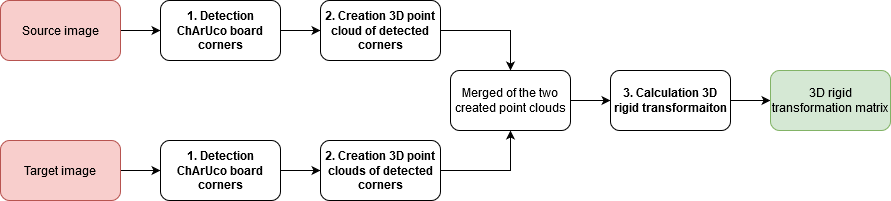
\includegraphics[width=0.95\textwidth]{images/registration/registration.png}
    \caption{Pipeline of the proposed method to find the rigid tranformation matrix}
    \label{figure:registration}
\end{figure}

\subsubsection{Detection of a ChArUco board corners}
\label{section:charuco_board_corners}
To obtain a precise registration, accurate and easy to detect keypoints have to be recognised in the field of view of the different cameras. ArUco markers and chessboards are very useful due to their fast detection and their versatility. The algorithm to detect the corners of the chessboard was developed by \cite{harris_combined_1988}.

The detection and generation of ArUco markers were developed by \cite{garrido-jurado_automatic_2014}. ArUco markers have the advantage of having a unique identification number by pattern. It makes ArUco board versatile and permissive to occlusion. Therefore matching these markers viewed by different cameras is straightforward. On the other hand, the accuracy of their corner positions is not high enough \footnote{According to the OpenCv documentation: \url{https://docs.opencv.org/4.2.0/df/d4a/tutorial_charuco_detection.html}}.

By comparing with ArUco markers, the corners of chessboard patterns can be refined more accurately. Each corner is surrounded by two squares which increases the accuracy of the corner position. However, such a board is less versatile and is not permissive to occlusion.

The benefits of these two different boards are combined in a ChArUco board, figure \ref{figure:charucodefinition}. OpenCV library is used to handle the detection of the corners.

\begin{figure}[H]
    \centering
    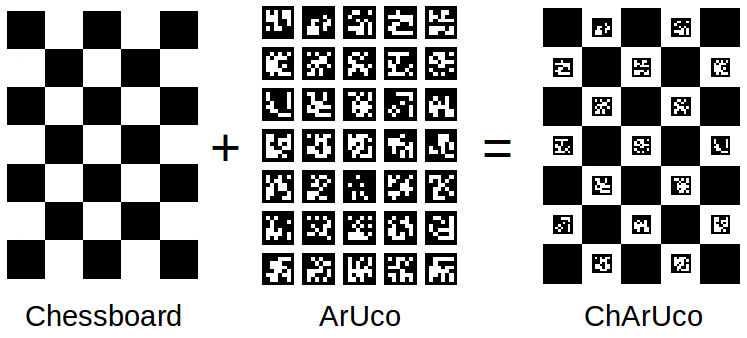
\includegraphics[width=0.65\textwidth]{images/registration/charucodefinition.png}
    \caption{ChArUco board definition}
    \label{figure:charucodefinition}
\end{figure}

A tripod with a ChArUco board is placed in the centre of the scene. It has to be in the field of view of both cameras. The positions in pixel of the detected chessboard corners are recorded for both views. The average over about 50 frames is calculated to be robust to outliers and is saved for the second step.

\begin{figure}[H]
\centering
  \begin{subfigure}[b]{0.48 \textwidth}
    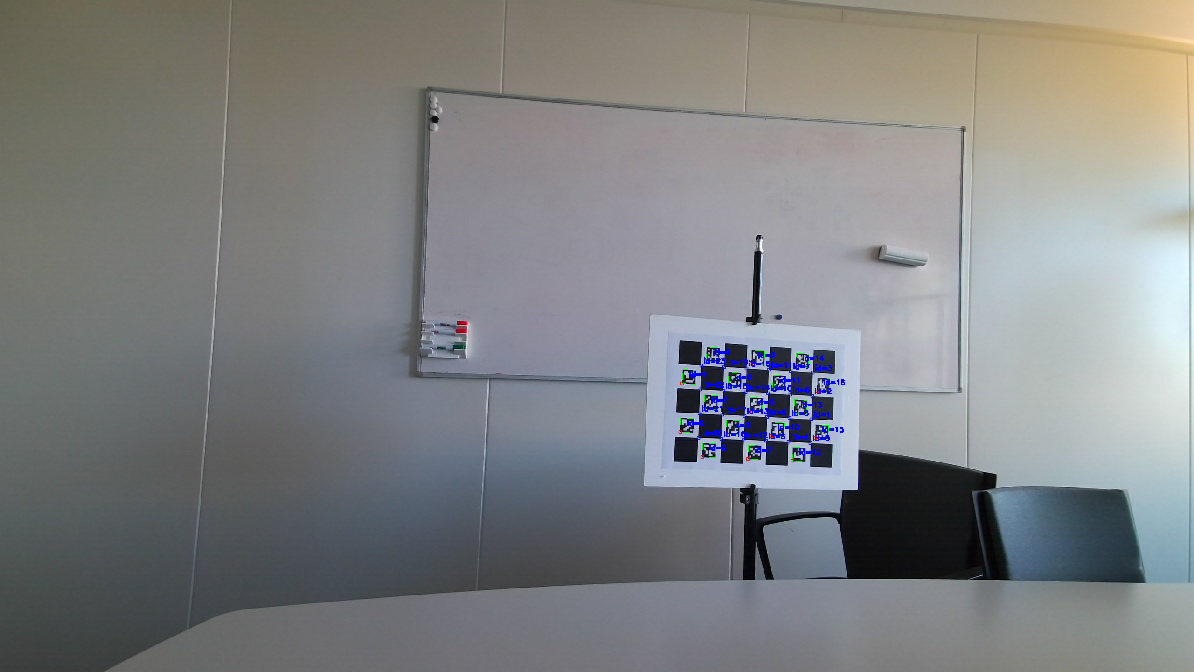
\includegraphics[width=\textwidth]{images/registration/imgr_board_detected.png}
    \caption{Chessboard detection on the right}
    \label{figure:imgr_board_detected}
  \end{subfigure}
  \hfill
  \begin{subfigure}[b]{0.48 \textwidth}
    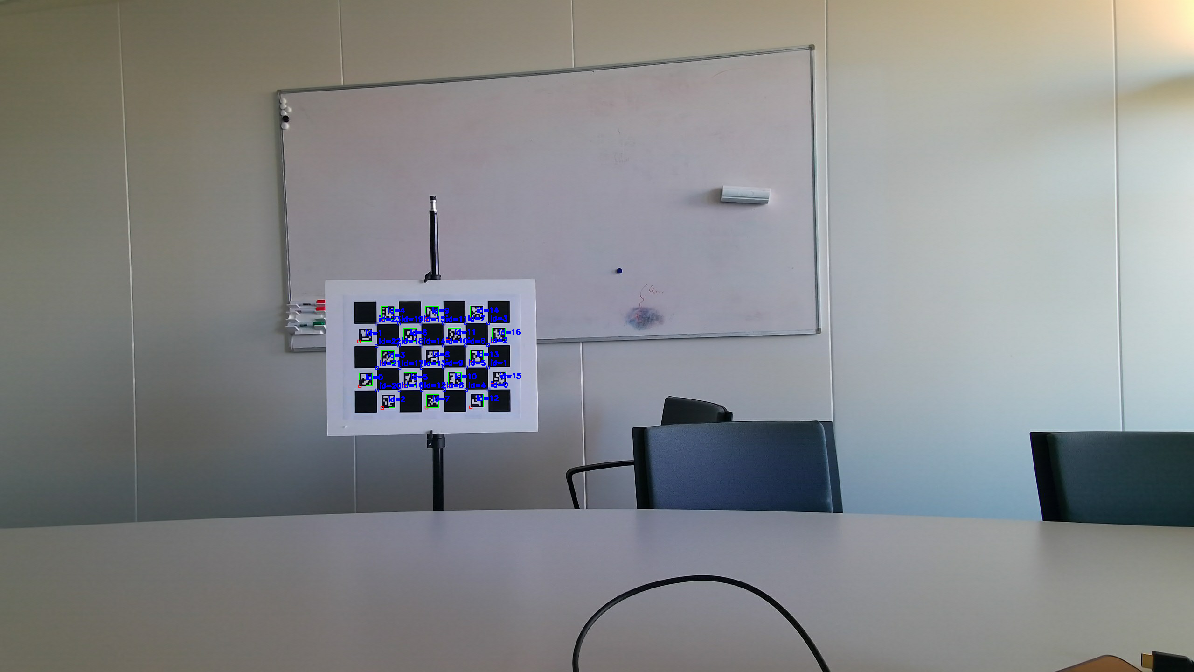
\includegraphics[width=\textwidth]{images/registration/imgl_board_detected.png}
    \caption{Chessboard detection on the left}
    \label{figure:imgl_board_detected}
  \end{subfigure}
  \caption{Detection of the chessboard corners from different position}
  \label{figure:img_board_detected}
\end{figure}


\subsubsection{Creation of a 3D point cloud of the detected corners}
\label{section:creation_3d_pc_corners}

In this second phase, the recorded positions of the corners and the depth images are used to create two 3D point clouds.

Given depth value d at (u, v) image coordinate, the corresponding 3D point is computed as follow thanks to the equation provided by\cite{Zhou2018}:

\begin{equation}
\label{equation:2dTO3d}
    \begin{array}{l}
        {z=d / c} \\
        {x=(u-c _ { x }) \cdot z / f _ { x }} \\
        {y=(v-c _ { y }) \cdot z / f _ { y }}
    \end{array}
\end{equation}
where:
\begin{itemize}
    \item $( x , y , z )$ are the coordinate of a 3D point in the corresponding camera space in a metric scale
    \item $( u , v )$ are the image coordinates
    \item $( c _ { x }, c _ { y })$ is a principal point that is usually at the image center expressed in pixel units.
    \item $ f _ { x }, f _ { y }$ are the focal lengths expressed in pixel units.
    \item $c$ is the depth scale
\end{itemize}
\leavevmode\newline
$c _ { x }, c _ { y }, f _ { x }, f _ { y }$ are the intrinsic parameters of a camera. They are different for each camera and depends of the physic of the lens. They change regarding the chosen resolution. Microsoft provides these intrinsic parameters.

The formula (\ref{equation:2dTO3d}) is applied to all the 24 detected corners in order to create a point cloud. It is done for each camera separately. Figure \ref{figure:pc_arucoboard} shows the two resulting point clouds in the same coordinate space. They are used in the next step.

\begin{figure}[H]
    \centering
    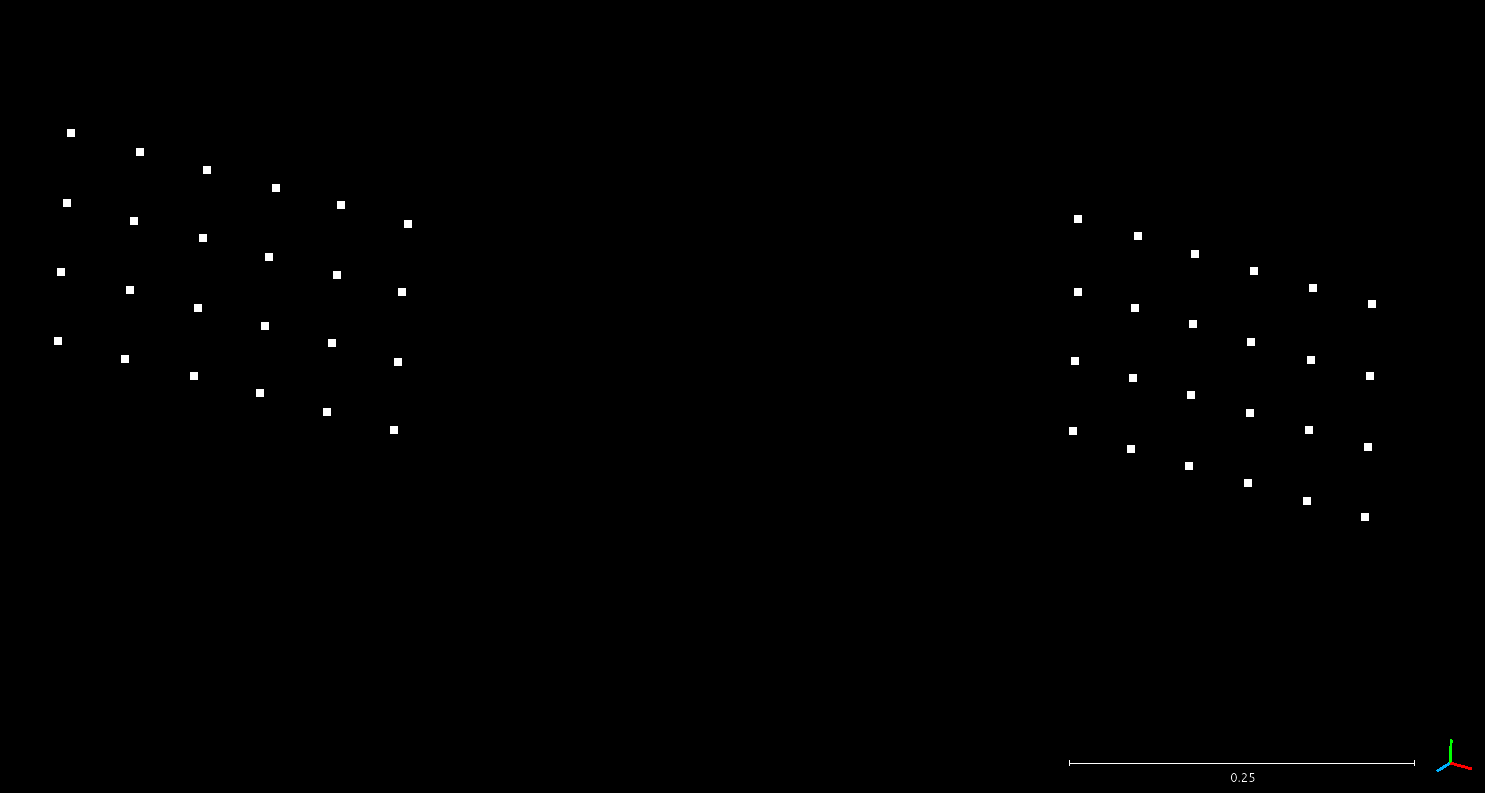
\includegraphics[width=0.65\textwidth]{images/registration/pc_aruco_24.png}
    \caption{Point cloud of the ChArUco board corners seen from the two cameras}
    \label{figure:pc_arucoboard}
\end{figure}


\subsubsection{Calculation of a 3D  rigid transformation}
\label{section:3d_rigid_transformation}

The last step consists of finding the rigid transformation to align the ChArUco board corners point clouds of the two different views. Once this matrix is found, it can be applied to the whole scene as long as the position of the cameras is not changing. The whole pipeline has to be repeated if the position of the cameras is changed. This matrix is calculated via a function\footnote{$compute\_transformation$ of the class $open3d.registration.TransformationEstimationPointToPoint$}
 provided by the library Open3D \cite{Zhou2018}. This function uses an algorithm based on \cite{umeyama_least-squares_1991}. It estimates parameters $c, \mathbf{R}$ and $\mathbf{t}$ such that the following equation is minimised:
 
%  \begin{align*}
%      \frac{1}{n} \sum_{i=1}^n\vert\vert y_i - (c\mathbf{R}x_i + \mathbf{t})\vert\vert_2^2
%  \end{align*}
 
 \begin{equation}
    \frac{1}{n} \sum_{i=1}^{n}\left\|y_{i}-\left(c \mathbf{R} x_{i}+\mathbf{t}\right)\right\|_{2}^{2}
\end{equation}

Singular value decomposition (SVD) is used by \cite{umeyama_least-squares_1991} to minimise this equation
 

% \todo{https://eigen.tuxfamily.org/dox/group__Geometry__Module.html#gab3f5a82a24490b936f8694cf8fef8e60}


% $compute\_transformation$ of the class $open3d.registration.TransformationEstimationPointToPoint$ provided by the library Open3D \cite{noauthor_open3d_nodate} is used to calculate this transformation matrix.
\subsection{Results}
The purpose of this section is to compare some of the different methods mentioned in the previous section \nameref{section:registration_previous_work}. Each of these methods produces a different transformation matrix. They are all applied on the point clouds created from the ChArUco board corners, see figure \ref{figure:pc_arucoboard}. It is supposed that a perfect transformation matrix should align exactly both point clouds. The mean absolute error is calculated for each point to estimate the error of each method. The steps for all experiments are the following:

\begin{enumerate}
    \item Estimate the rigid transformation matrix
    \item Transform one view into the other one with the estimated transformation matrix
    \item Calculate the mean absolute error (MAE) between the matching points of the ChArUco board of both views in each direction. The definition of the coordinates was presented in section \ref{section:3D coordinate system}.
\end{enumerate}

\subsubsection{Global registration}
\label{section:Global registration result}
\textbf{Experiment 1}

In this experiment, the procedure presented in section \ref{section:Global registration} is applied. A selected frame of the static scene is chosen. The two point clouds of the two different views are created. Without any transformation, the scene looks like in figure \ref{figure:pc_raw_static_merged}

\begin{figure}[H]
\centering
  \begin{subfigure}[b]{0.48 \textwidth}
    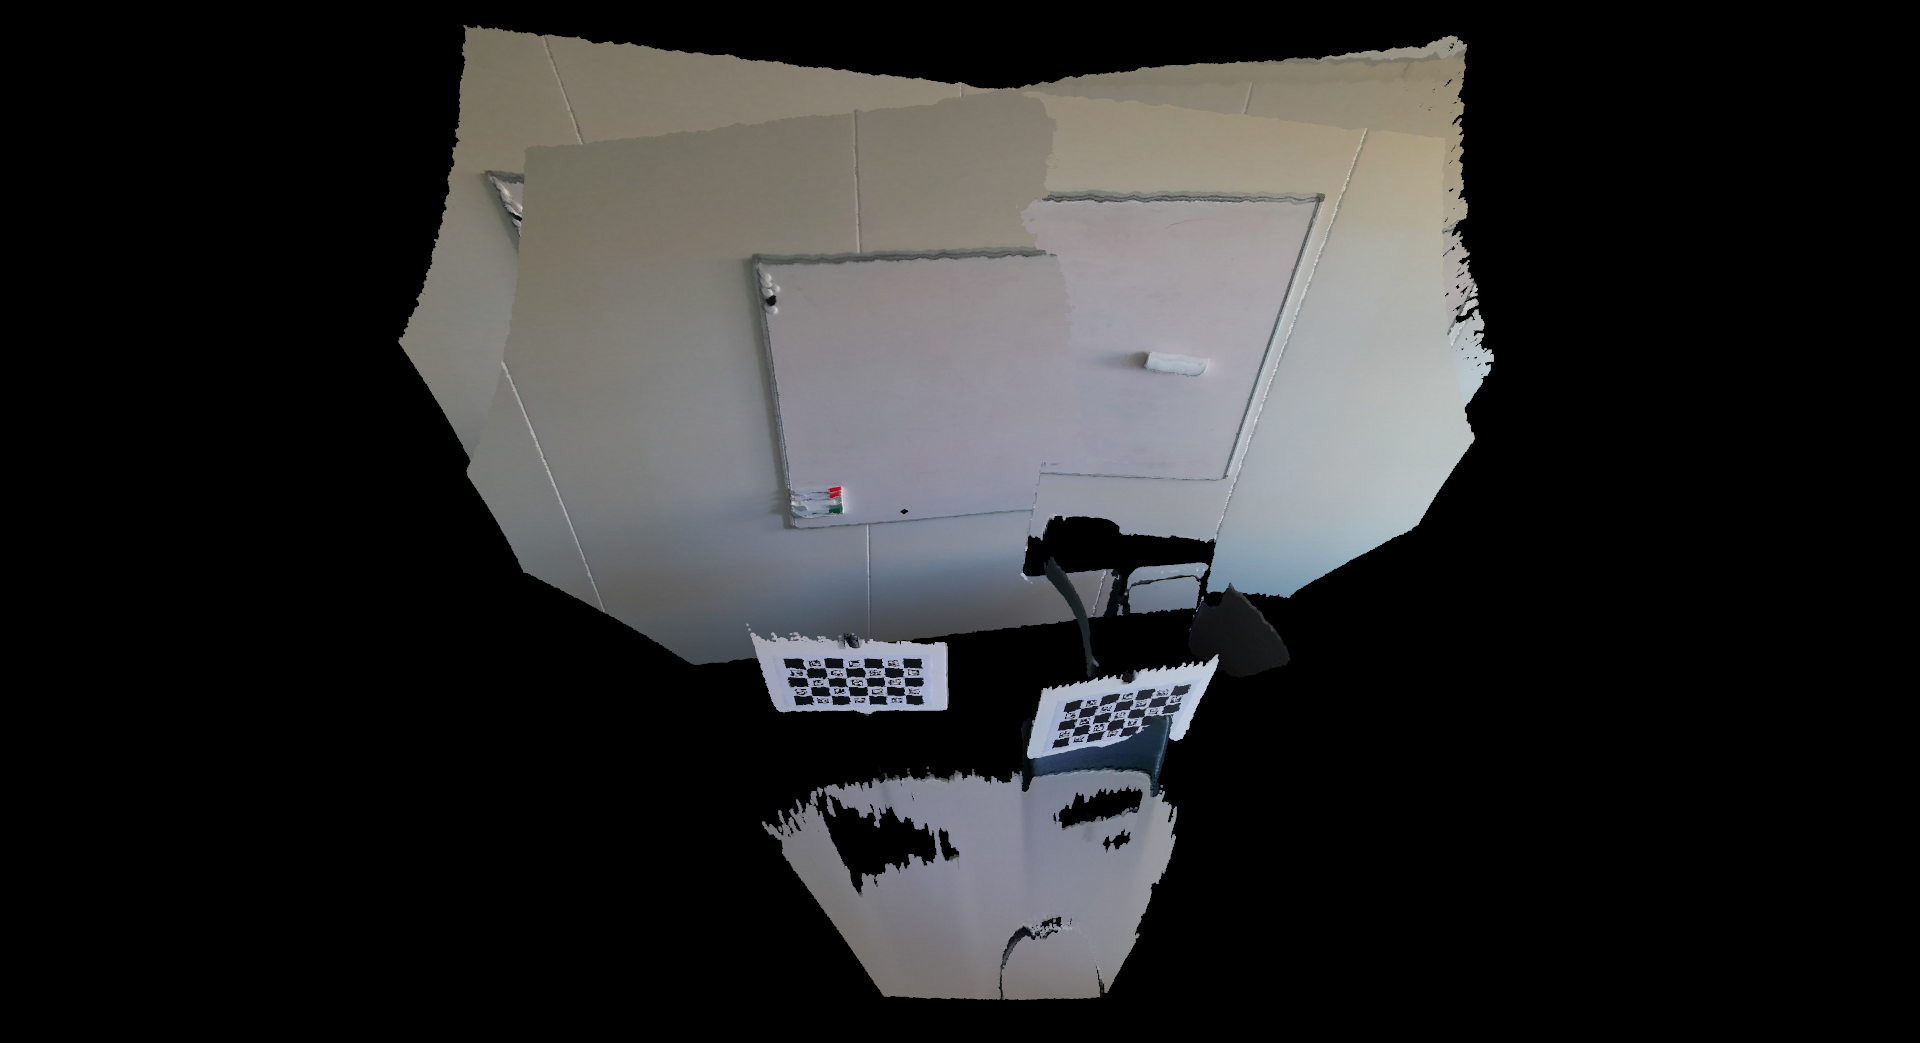
\includegraphics[width=\textwidth]{images/registration/pc_raw_static_merged_rgb.png}
    \caption{Merge of the two point clouds in RGB}
    \label{figure:pc_raw_static_merged_rgb}
  \end{subfigure}
  \hfill
  \begin{subfigure}[b]{0.48 \textwidth}
    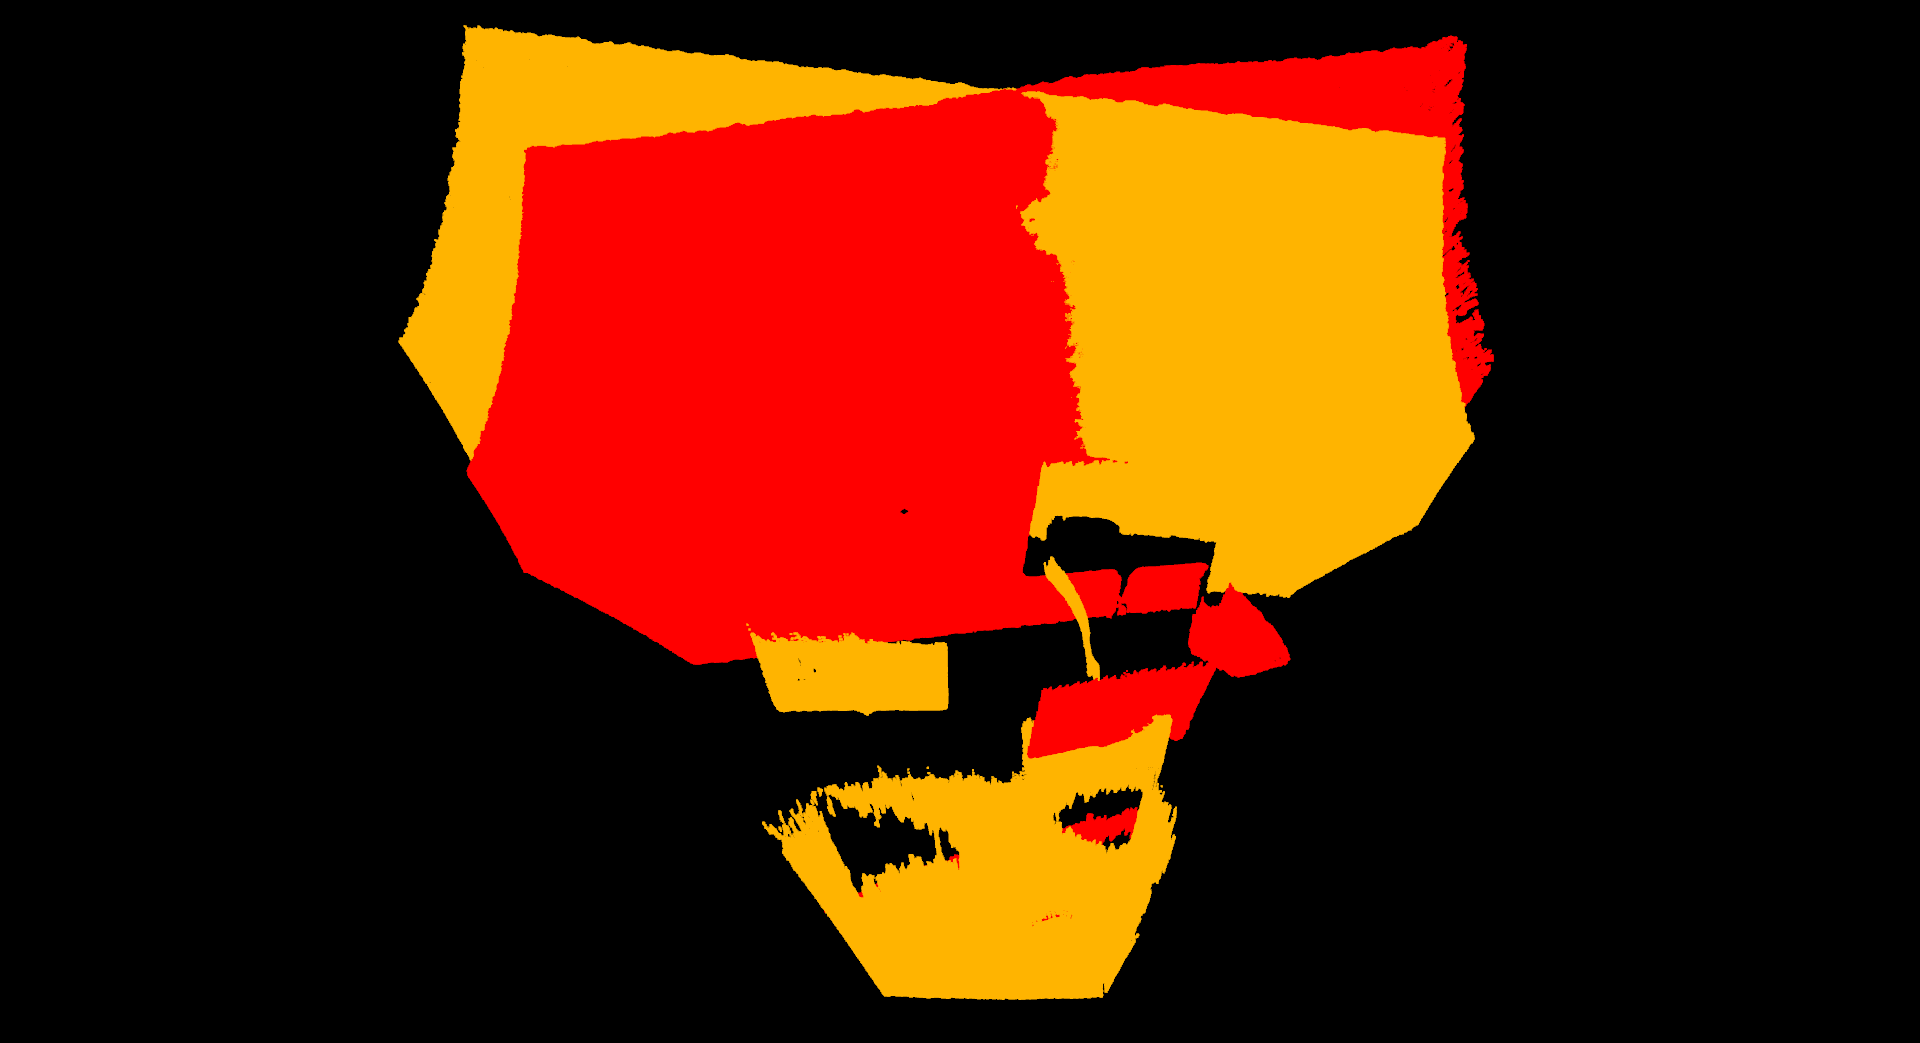
\includegraphics[width=\textwidth]{images/registration/pc_raw_static_merged_color.png}
    \caption{Red: point cloud 1. Yellow: point cloud 2.}
    \label{figure:pc_raw_static_merged_color}
  \end{subfigure}
  \caption{Merge of the two point clouds created from the two different views before applying any transformation. The point of view is virtual.}
  \label{figure:pc_raw_static_merged}
\end{figure}

Global registration procedure failed to find any transformation matrix to align the two point clouds of figure \ref{figure:pc_raw_static_merged}. One  reason could be the difficulty for FPFH to find relevant feature to process the alignment. As FPFH describes the local geometry property of a point, this property could be too much similar with point clouds having big planar surfaces.

\textbf{Experiment 2}

Applying the same procedure on the same scene but without the background (i.e. the wall) gives some results for the transformation matrix. The problem is that each time the global registration procedure is executed, the resulting output is extremely different and gives rarely a good result (about 1/20), see figure \ref{figure:ransac}. The reason is the RANSAC step where point are picked randomly and also because FPFH gives too similar local geometry properties.

\begin{figure}[H]
\centering
  \begin{subfigure}[b]{0.48 \textwidth}
    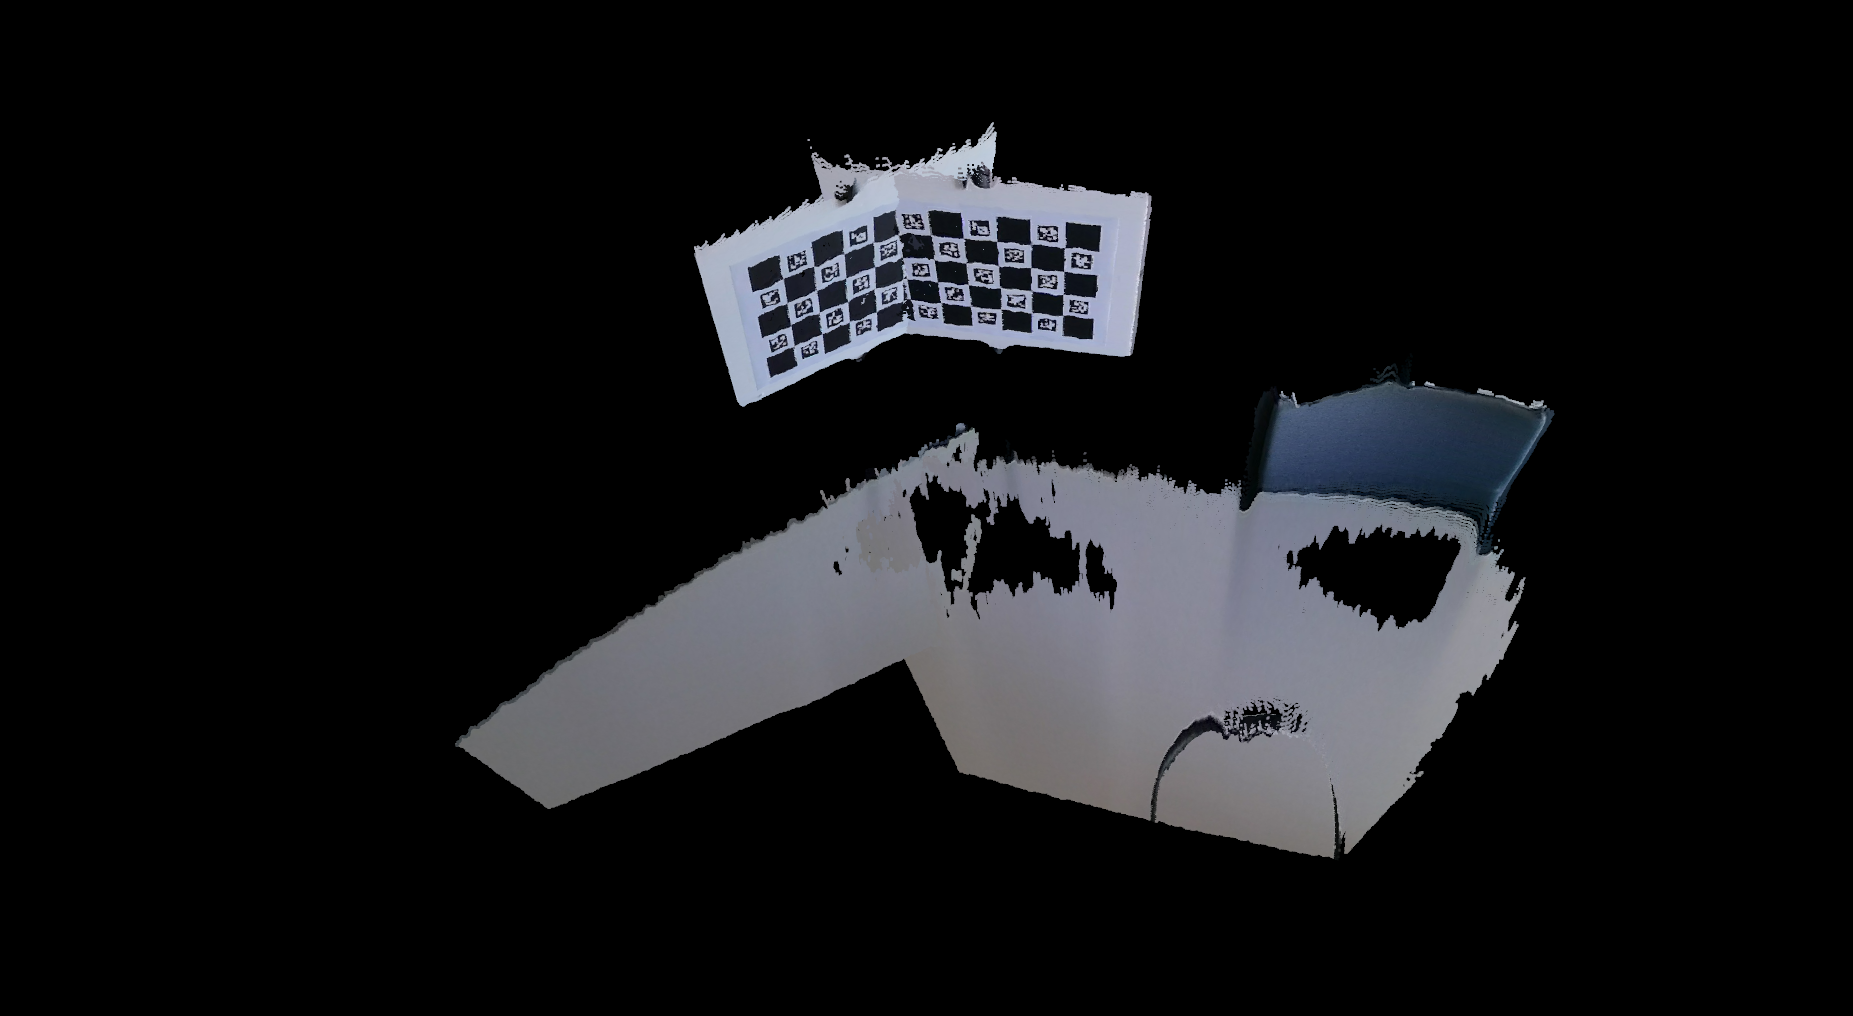
\includegraphics[width=\textwidth]{images/registration/ransac0.png}
    \caption{Example 1}
    \label{figure:ransac0}
  \end{subfigure}
  \hfill
  \begin{subfigure}[b]{0.48 \textwidth}
    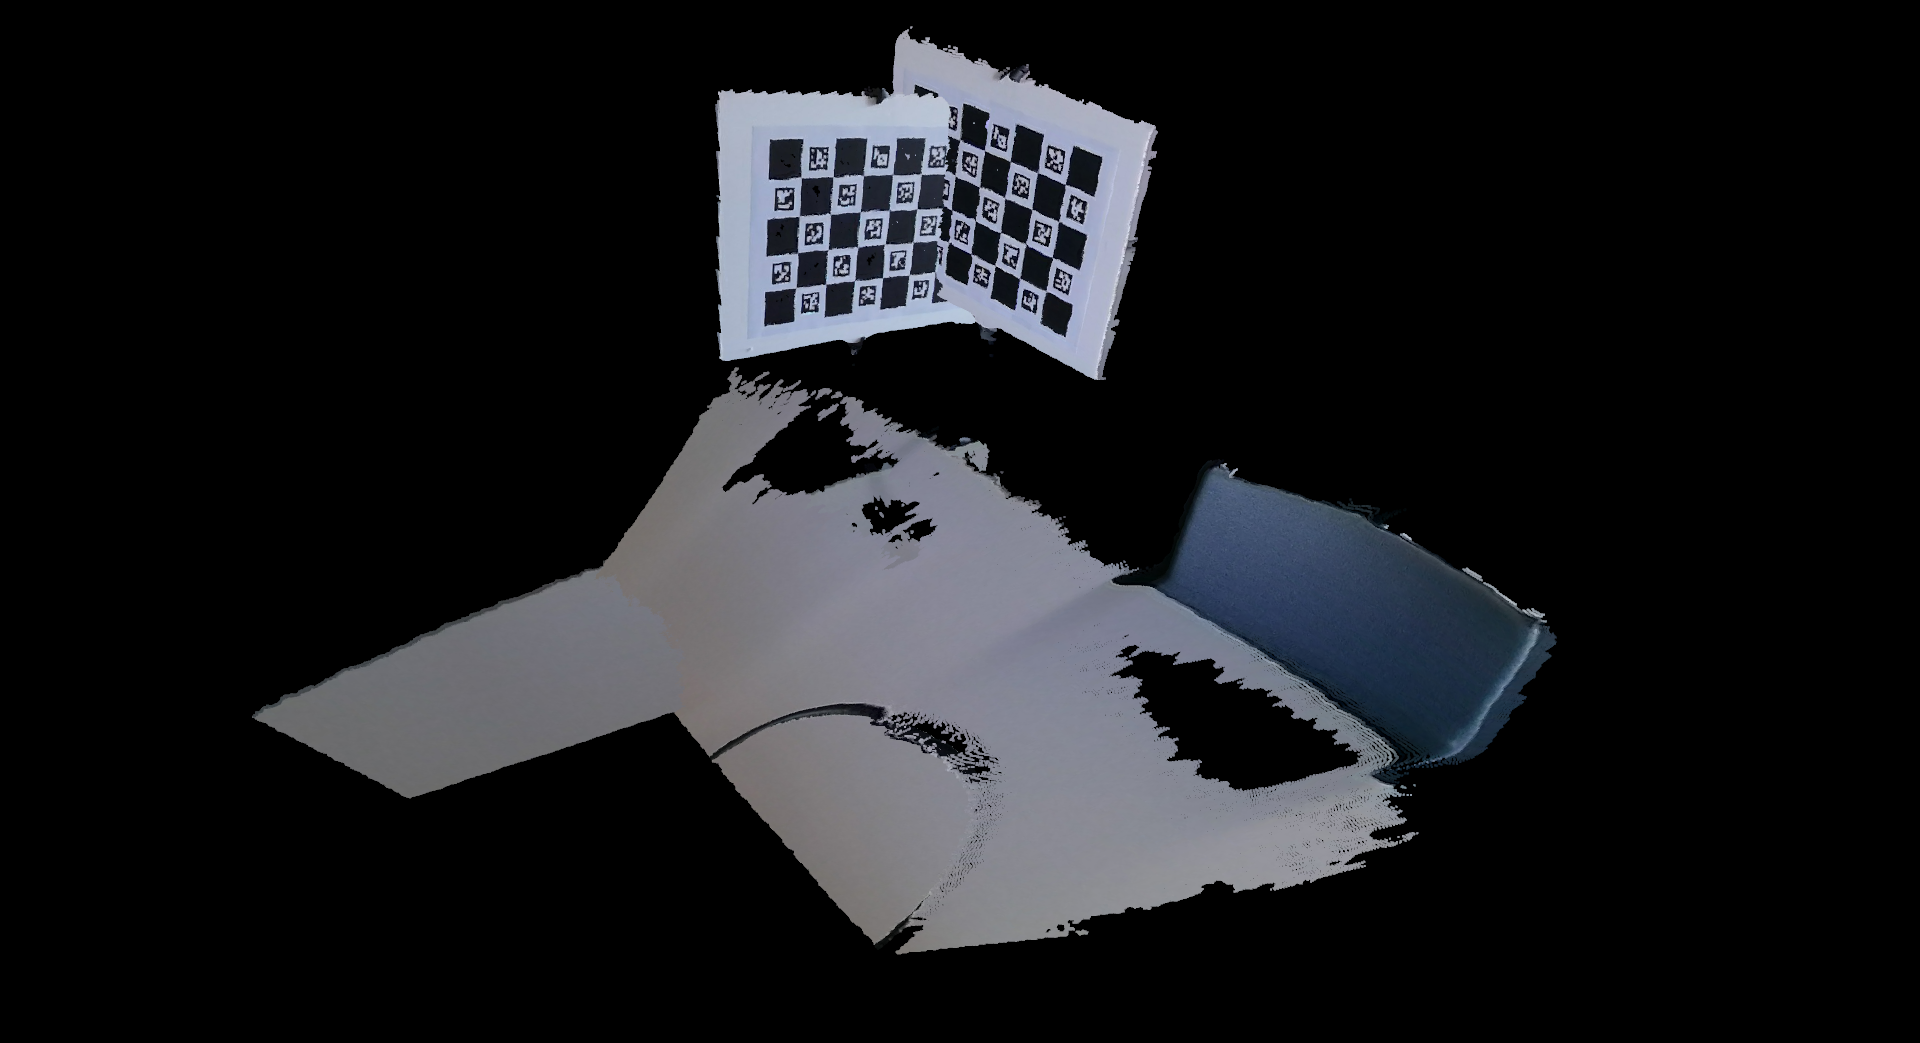
\includegraphics[width=\textwidth]{images/registration/ransac1.png}
    \caption{Example 2}
    \label{figure:ransac1}
  \end{subfigure}
  \caption{Sample of bad transformation matrix found by the global registration procedure}
  \label{figure:ransac}
\end{figure}

Figure \ref{figure:ransac_ok} shows an example where the global registration procedure succeeds to find an acceptable transformation matrix.

\begin{figure}[H]
\centering
  \begin{subfigure}[b]{0.48 \textwidth}
    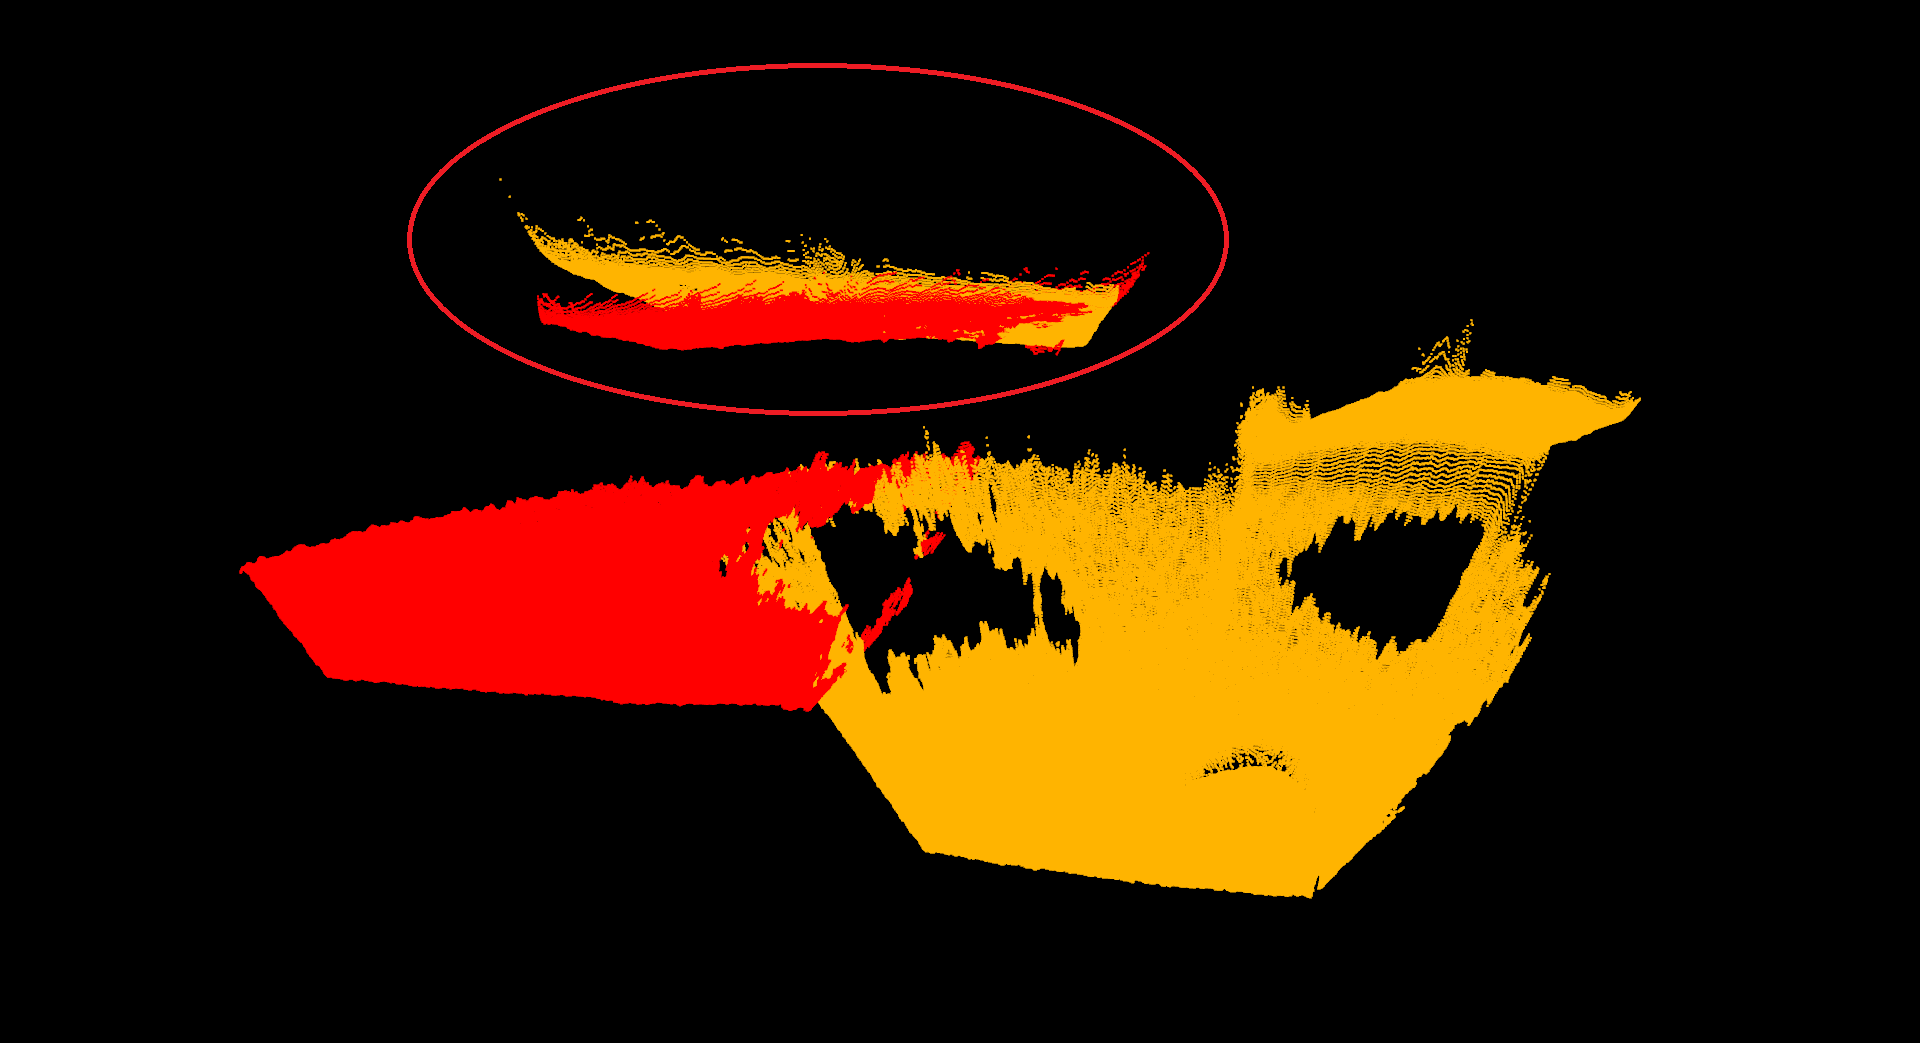
\includegraphics[width=\textwidth]{images/registration/ransac_ok_red.png}
    \caption{Result of the alignment after the RANSAC step}
    \label{figure:ransac_ok}
  \end{subfigure}
  \hfill
  \begin{subfigure}[b]{0.48 \textwidth}
    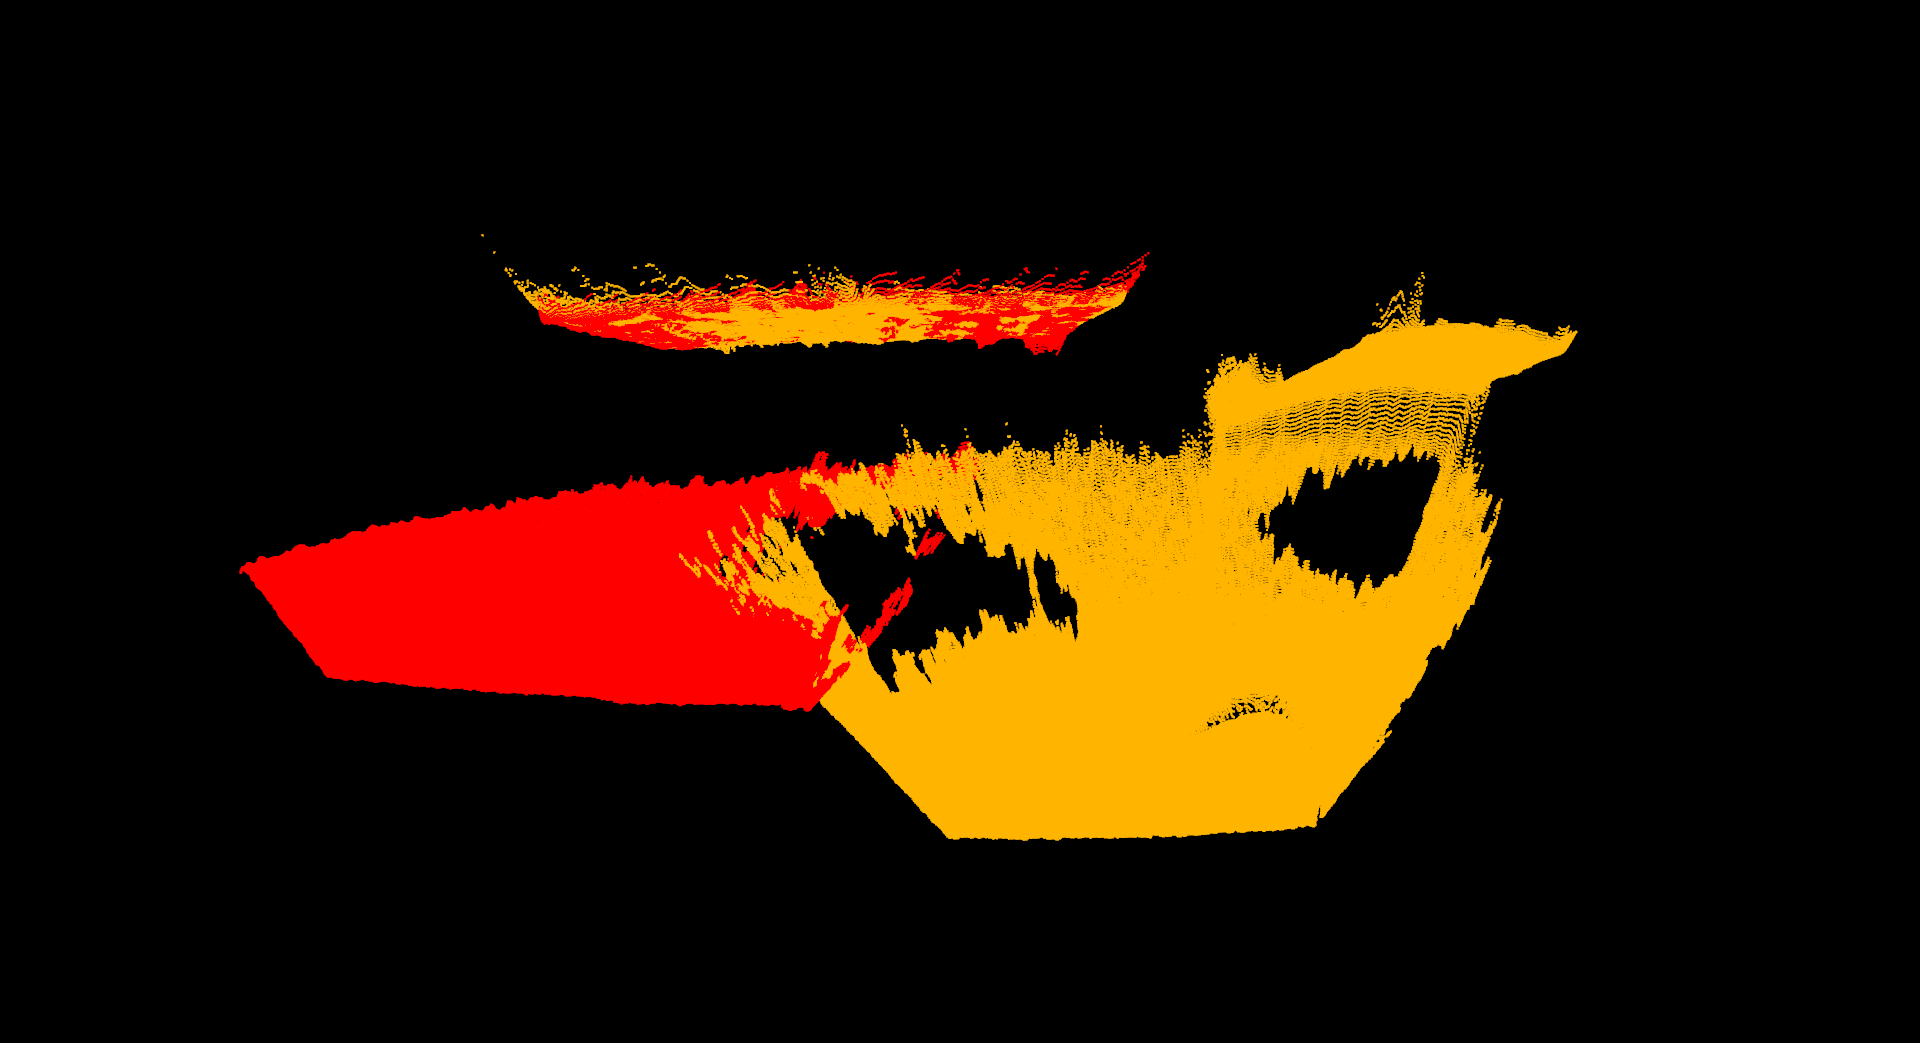
\includegraphics[width=\textwidth]{images/registration/ransac_icp_ok.png}
    \caption{Result of the alignment after the local refinement}
    \label{figure:ransac_icp_ok}
  \end{subfigure}
  \caption{Result of the global procedure on a sample without a wall as background. This is a virtual top view of the scene. Red: point cloud 1. Yellow: point cloud 2.}
  \label{figure:ransac_ok}
\end{figure}

Table \ref{tab:mae_global_registration_exp1} presents the result of applying the found transformation matrices on the  ChArUco board corners point clouds. It shows a non negligible improvement after the local refinement step.

\begin{table}[H]
\centering
\begin{tabular}{c|c|c|c}
 & \textbf{X - coordinate} & \textbf{Y - coordinate} & \textbf{Z - coordinate} \\ \hline
\textbf{\begin{tabular}[c]{@{}c@{}}Mean Absolute Error after\\ the RANSAC step {[}mm{]}\end{tabular}} & 6.05 & 13.14 & 20.11 \\ \hline
\textbf{\begin{tabular}[c]{@{}c@{}}Mean Absolute Error after\\ the refinement step {[}mm{]}\end{tabular}} & 3.04 & 0.57 & 2.40
\end{tabular}
\caption{Mean absolute error for the global registration experiment}
\label{tab:mae_global_registration_exp1}
\end{table}

\textbf{Experiment 3}

For this experiment, a scene with less planar surfaces is used. A static subject is put in the middle of the scene. Figure \ref{figure:raw_myself} shows the initial situation. The wall in the background is removed.

\begin{figure}[H]
\centering
  \begin{subfigure}[b]{0.48 \textwidth}
    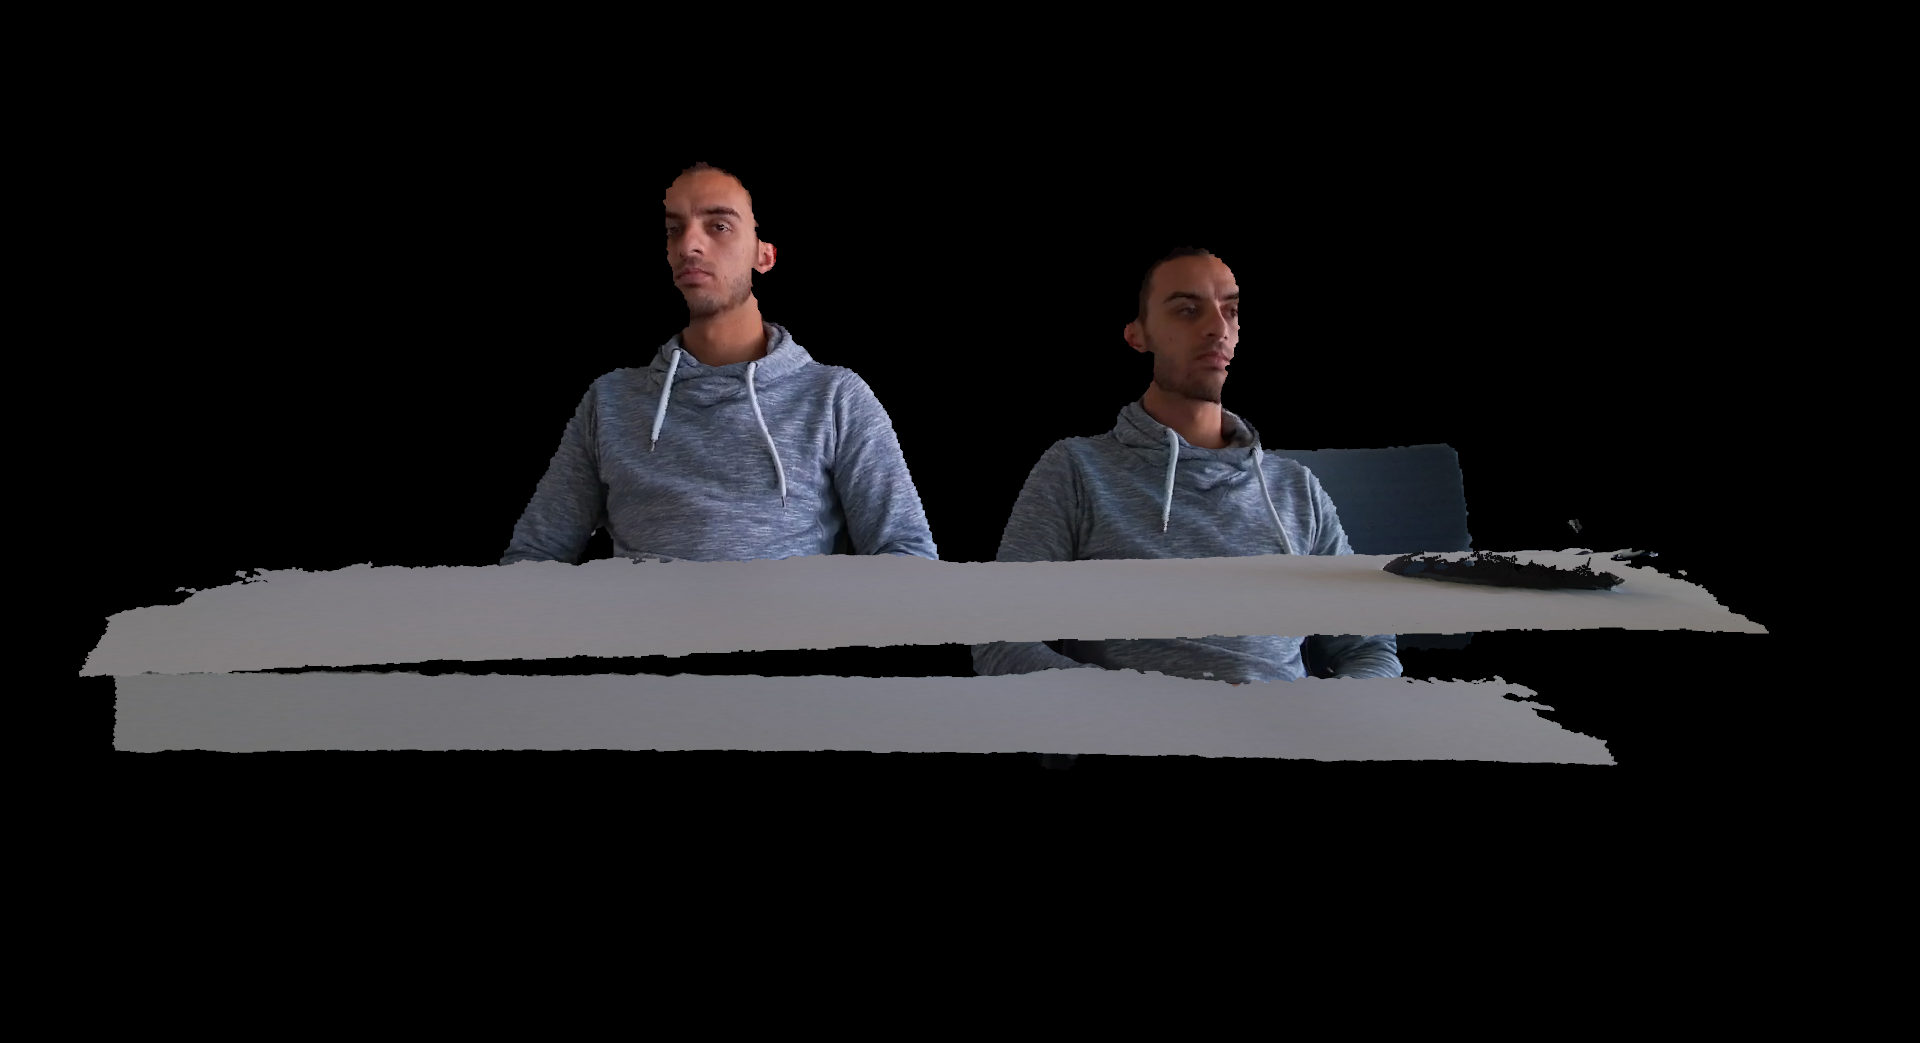
\includegraphics[width=\textwidth]{images/registration/raw_myself_RGB.png}
    \caption{RGB merged point clouds}
    \label{figure:raw_myself_RGB}
  \end{subfigure}
  \hfill
  \begin{subfigure}[b]{0.48 \textwidth}
    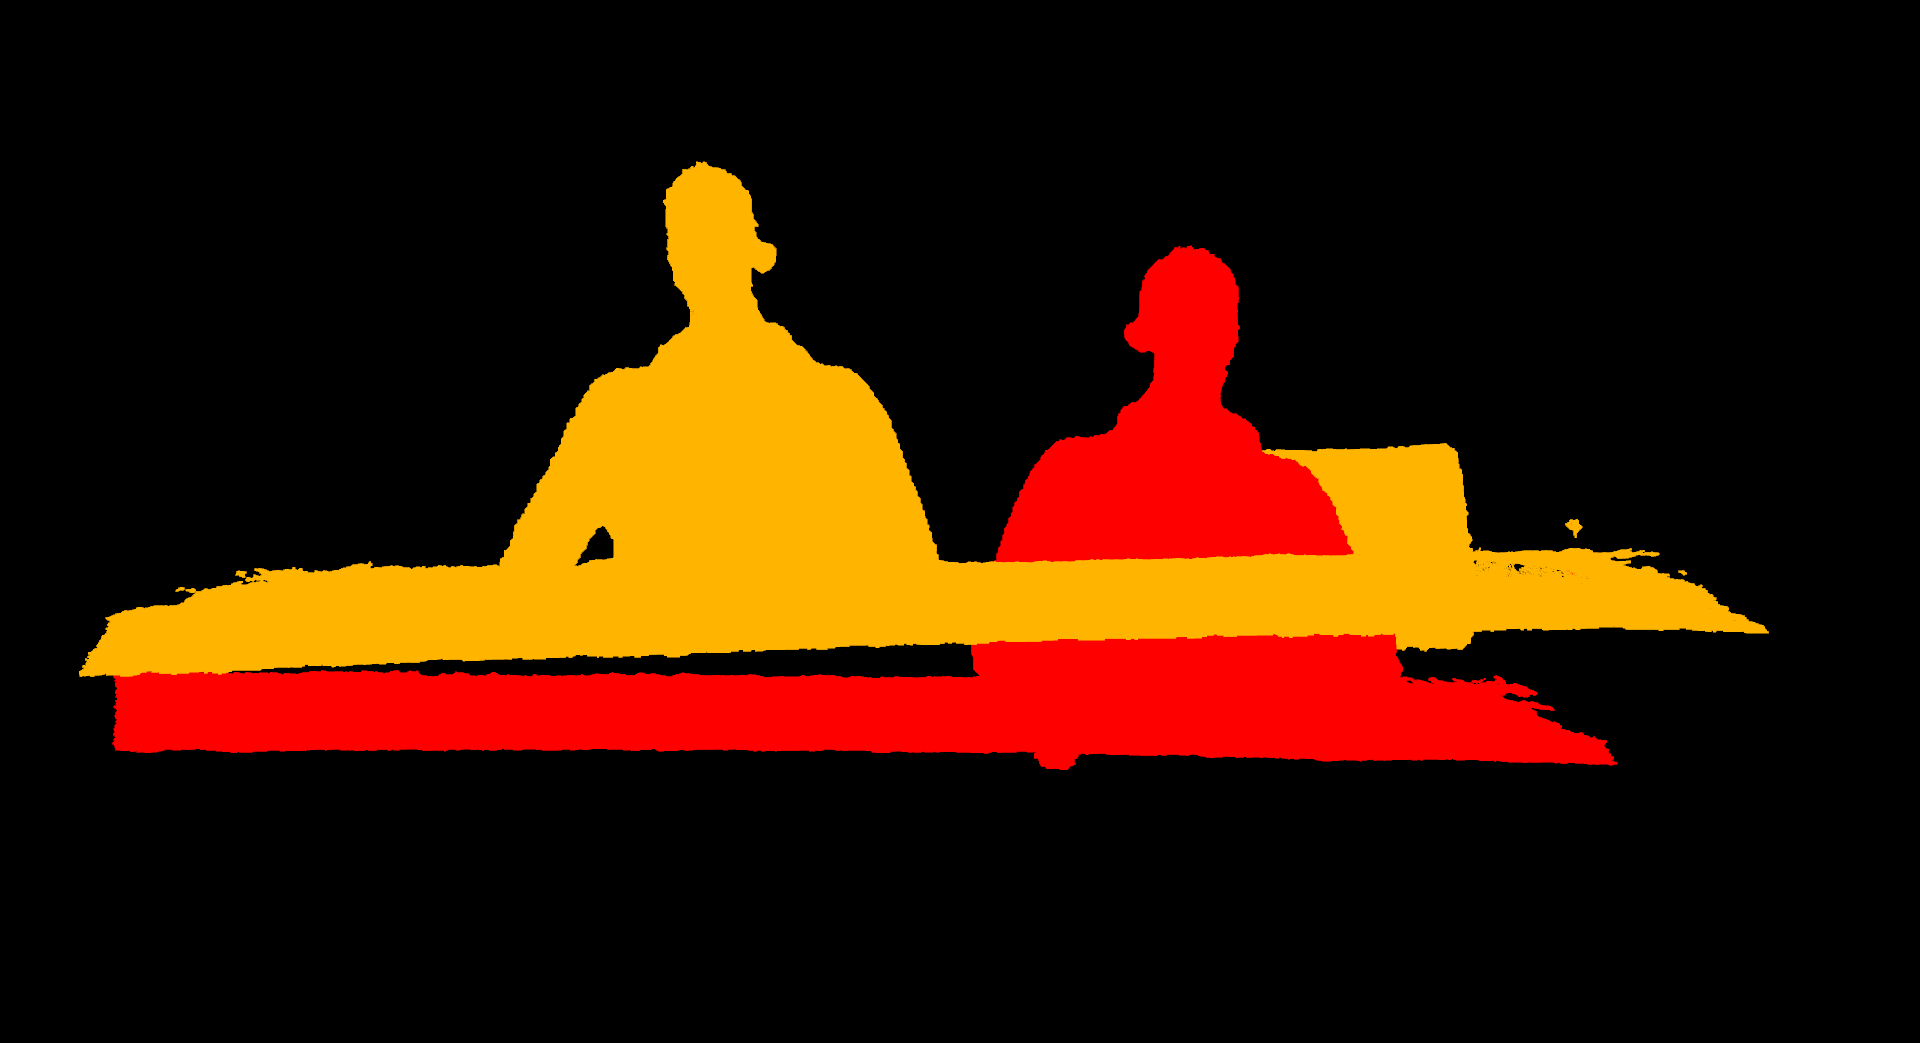
\includegraphics[width=\textwidth]{images/registration/raw_myself_colored.png}
    \caption{Red: point cloud 1. Yellow: point cloud 2.}
    \label{figure:raw_myself_colored}
  \end{subfigure}
  \caption{Merge of the two point clouds created from the two different views before applying any transformation. The point of view is virtual.}
  \label{figure:raw_myself}
\end{figure}

The global registration algorithm finds an acceptable transformation matrix each time. However, because of the randomness of the RANSAC step, the found transformation matrix is slightly different each time the procedure is launched. Figure \ref{figure:ransac_refine_myself_RGB} shows the alignment after the RANSAC step and the refinement step, respectively figure \ref{figure:ransac_myself_RGB} and \ref{figure:refine_myself_RGB}.

\begin{figure}[H]
\centering
  \begin{subfigure}[b]{0.48 \textwidth}
    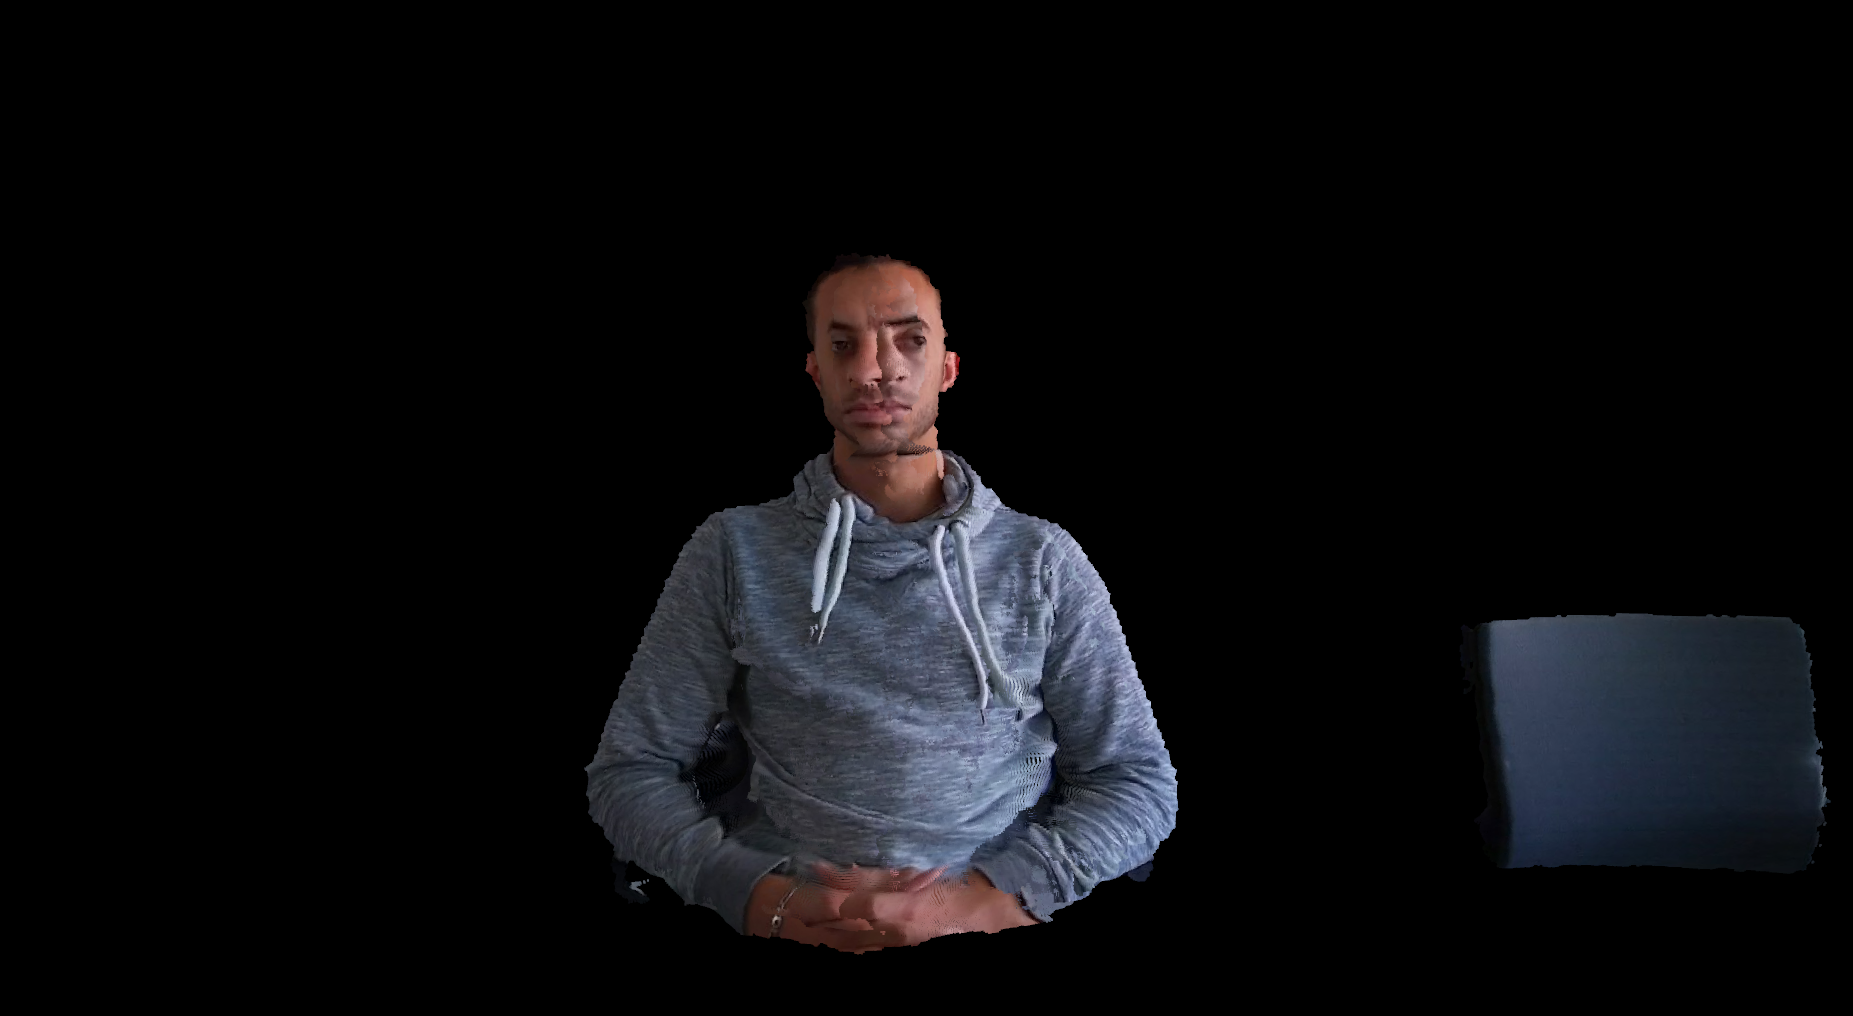
\includegraphics[width=\textwidth]{images/registration/ransac_myself_RGB.png}
    \caption{Alignment after the RANSAC step}
    \label{figure:ransac_myself_RGB}
  \end{subfigure}
  \hfill
  \begin{subfigure}[b]{0.48 \textwidth}
    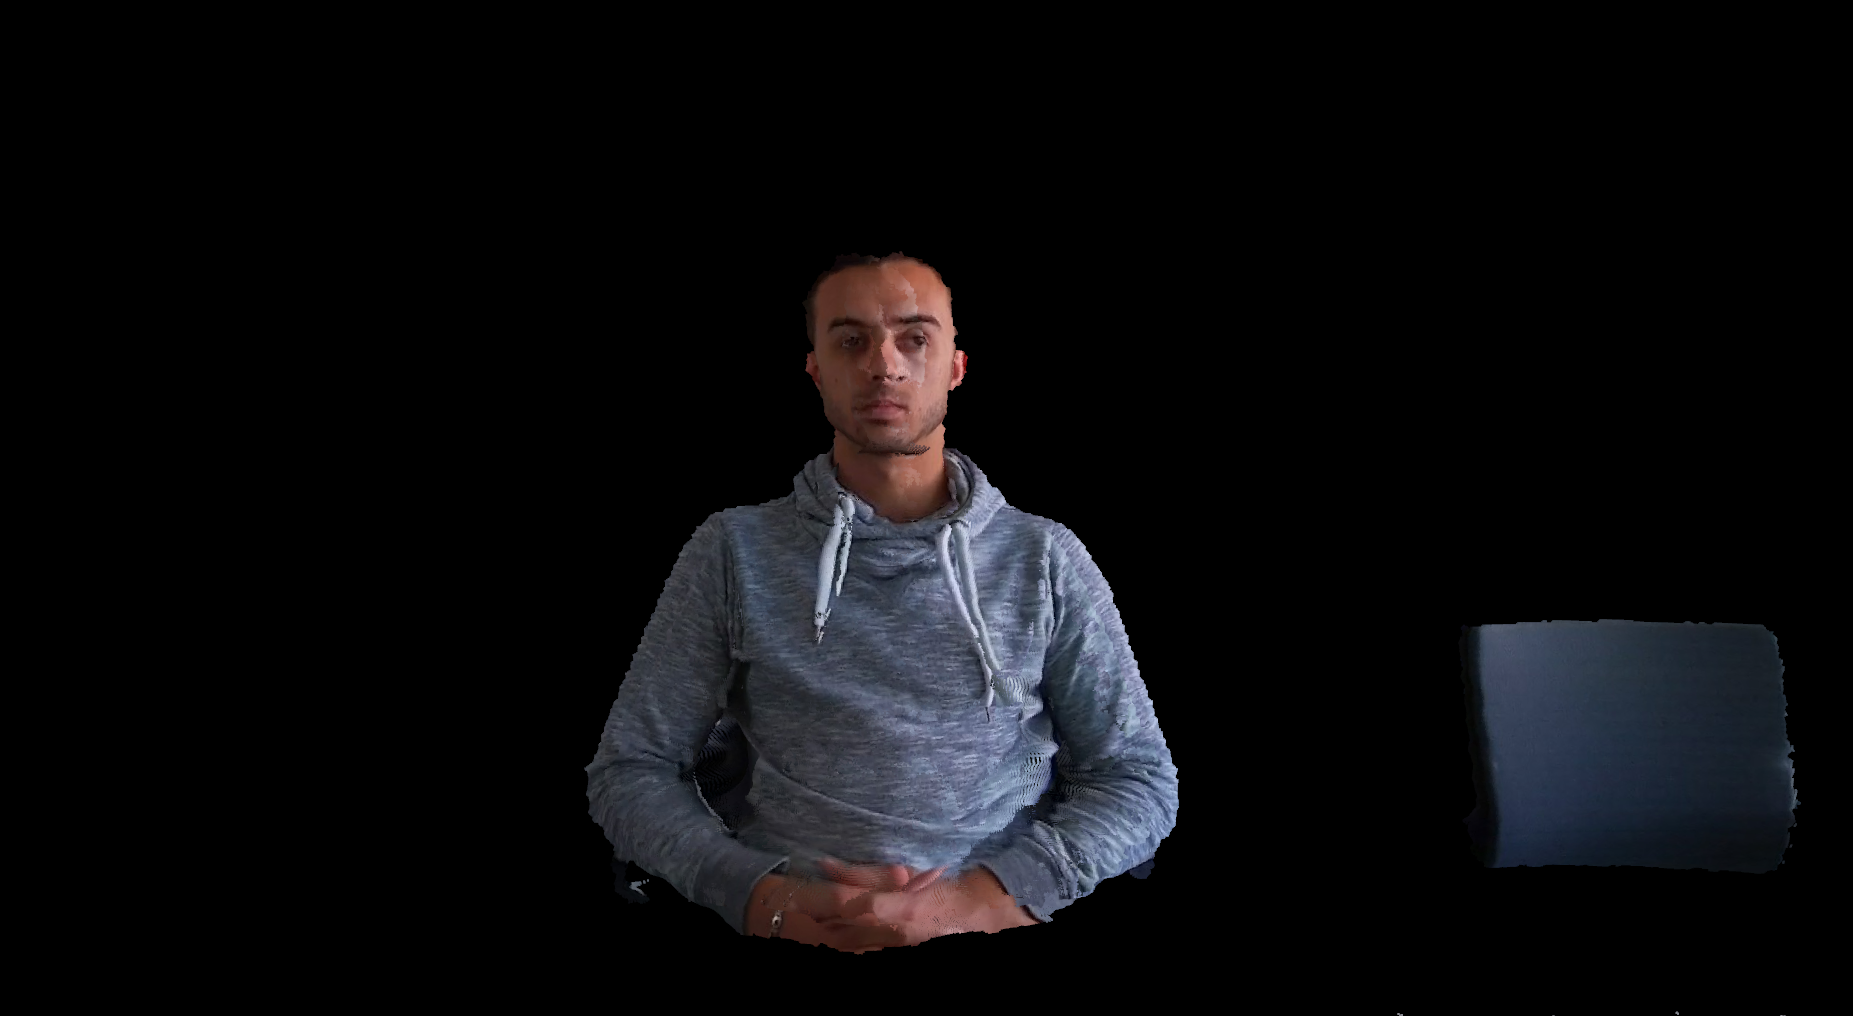
\includegraphics[width=\textwidth]{images/registration/refine_myself_RGB.png}
    \caption{Alignment after the refine step}
    \label{figure:refine_myself_RGB}
  \end{subfigure}
  \caption{Alignment of the two point clouds created from the two different views. The point of view is virtual.}
  \label{figure:ransac_refine_myself_RGB}
\end{figure}

Table \ref{tab:mae_global_registration_exp3} presents the results the three different matrices, found in the three previous experiments, applied on one of the ChArUco board point clouds of figure \ref{figure:pc_arucoboard}. One can notice that the result of the RANSAC step is not good enough to find an accurate transformation. The refinement step brings improvement. However, in this experiment, the MAE in \textit{X} is still high and noticeable in a live video demonstration. 


% Please add the following required packages to your document preamble:
% \usepackage{multirow}
\begin{table}[H]
\centering
\begin{tabular}{c|c|c|c|c}
 & \textbf{Run} & \textbf{X - coordinate} & \textbf{Y - coordinate} & \textbf{Z - coordinate} \\ \hline
\multirow{3}{*}{\textbf{\begin{tabular}[c]{@{}c@{}}Mean Absolute Error\\ after the RANSAC\\ step {[}mm{]}\end{tabular}}} & 1 & 30.67 & 4.07 & 3.66 \\
 & 2 & 19.93 & 0.87 & 2.62 \\
 & 3 & 29.51 & 0.62 & 5.42 \\ \hline
\multirow{3}{*}{\textbf{\begin{tabular}[c]{@{}c@{}}Mean Absolute Error\\ after the refinement\\  step {[}mm{]}\end{tabular}}} & 1 & 13.82 & 1.29 & 1.27 \\
 & 2 & 13.81 & 1.29 & 1.27 \\
 & 3 & 13.81 & 1.29 & 1.44
\end{tabular}
\caption{Mean absolute error for the global registration experiment}
\label{tab:mae_global_registration_exp3}
\end{table}


\subsubsection{Iterative closest point registration}

For all the ICP algorithms presented in section \ref{section:Iterative closest point registration}, the critical point is the guessed initialisation matrix. As is it difficult to estimate it, the transformation found after the RANSAC step of the experiment 2 of the section \ref{section:Global registration result} is used for the initialisation step.

\textbf{Experiment 1}

Figure \ref{figure:init_ransac} shows the scene after applying the RANSAC transformation found. All ICP algorithms are applied to this initial transformed scene.

\begin{figure}[H]
\centering
  \begin{subfigure}[b]{0.48 \textwidth}
    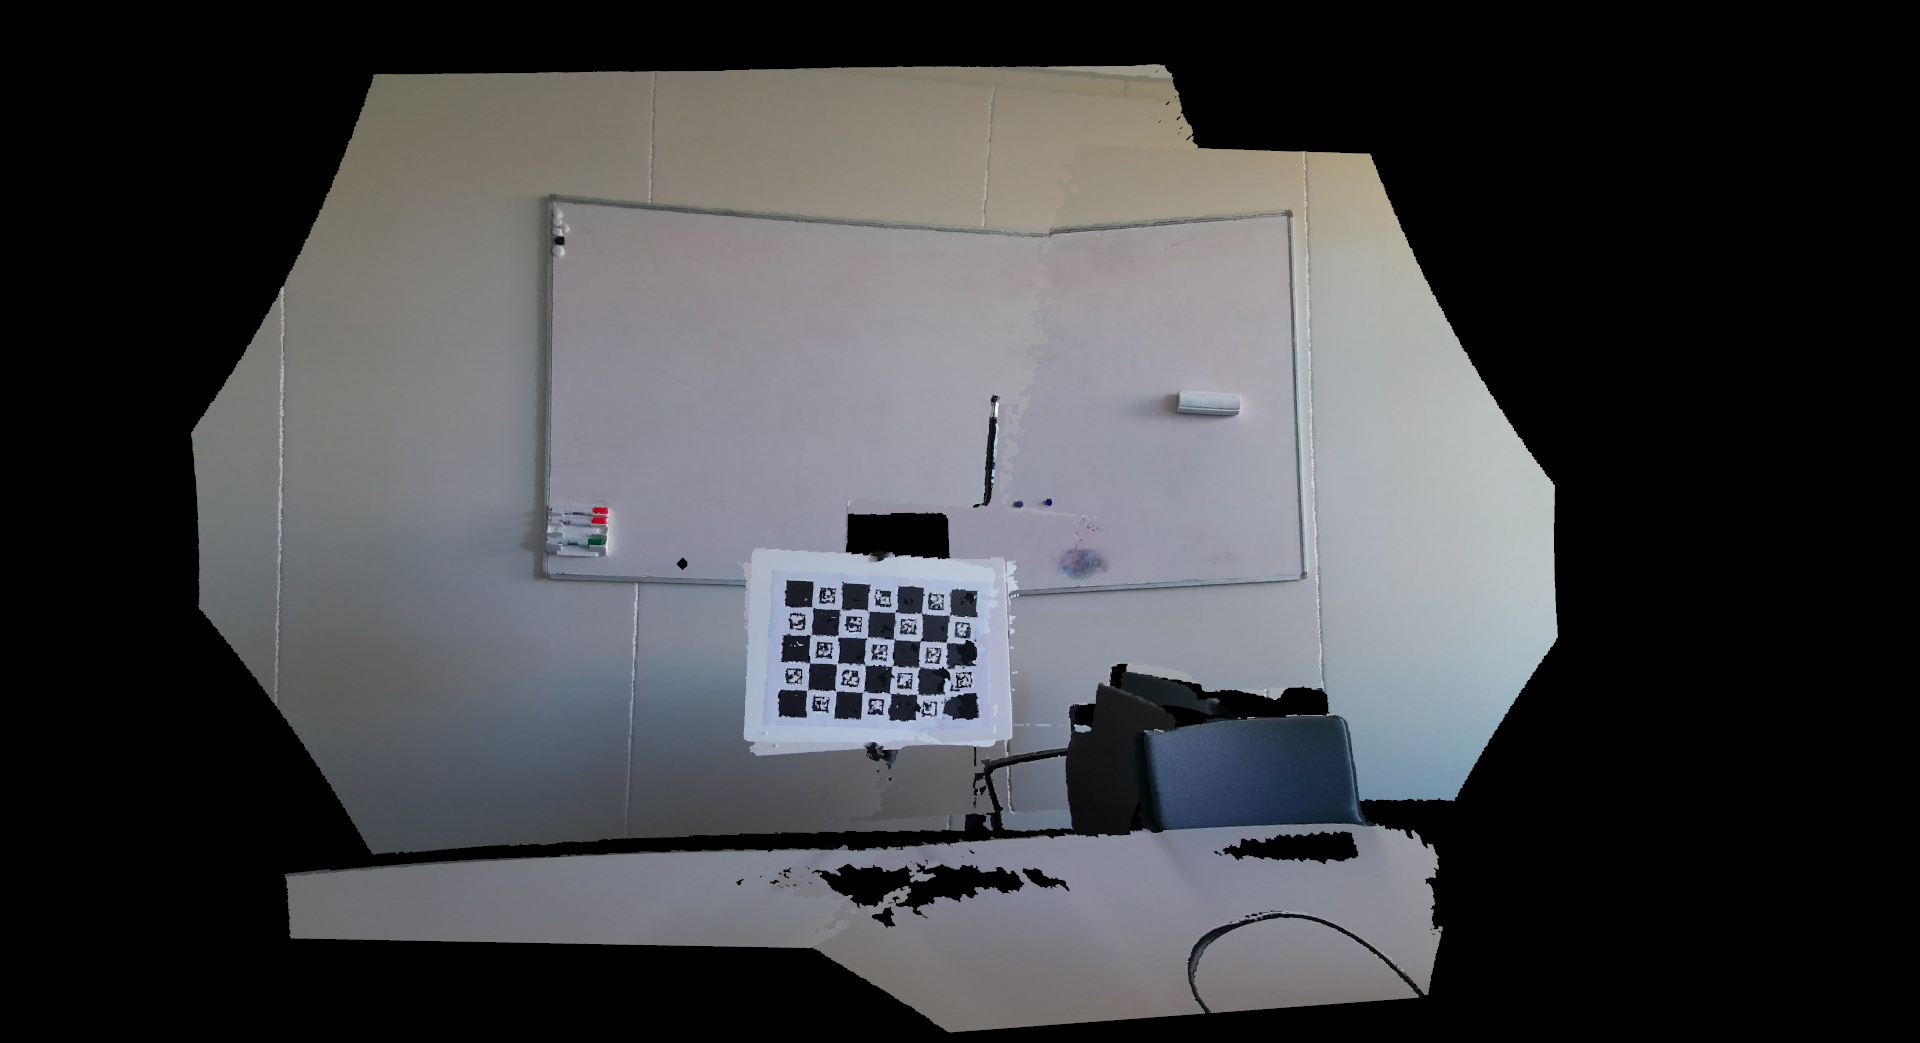
\includegraphics[width=\textwidth]{images/registration/init_ransac_RGB.png}
    \caption{Alignment after the RANSAC step}
    \label{figure:init_ransac_RGB}
  \end{subfigure}
  \hfill
  \begin{subfigure}[b]{0.48 \textwidth}
    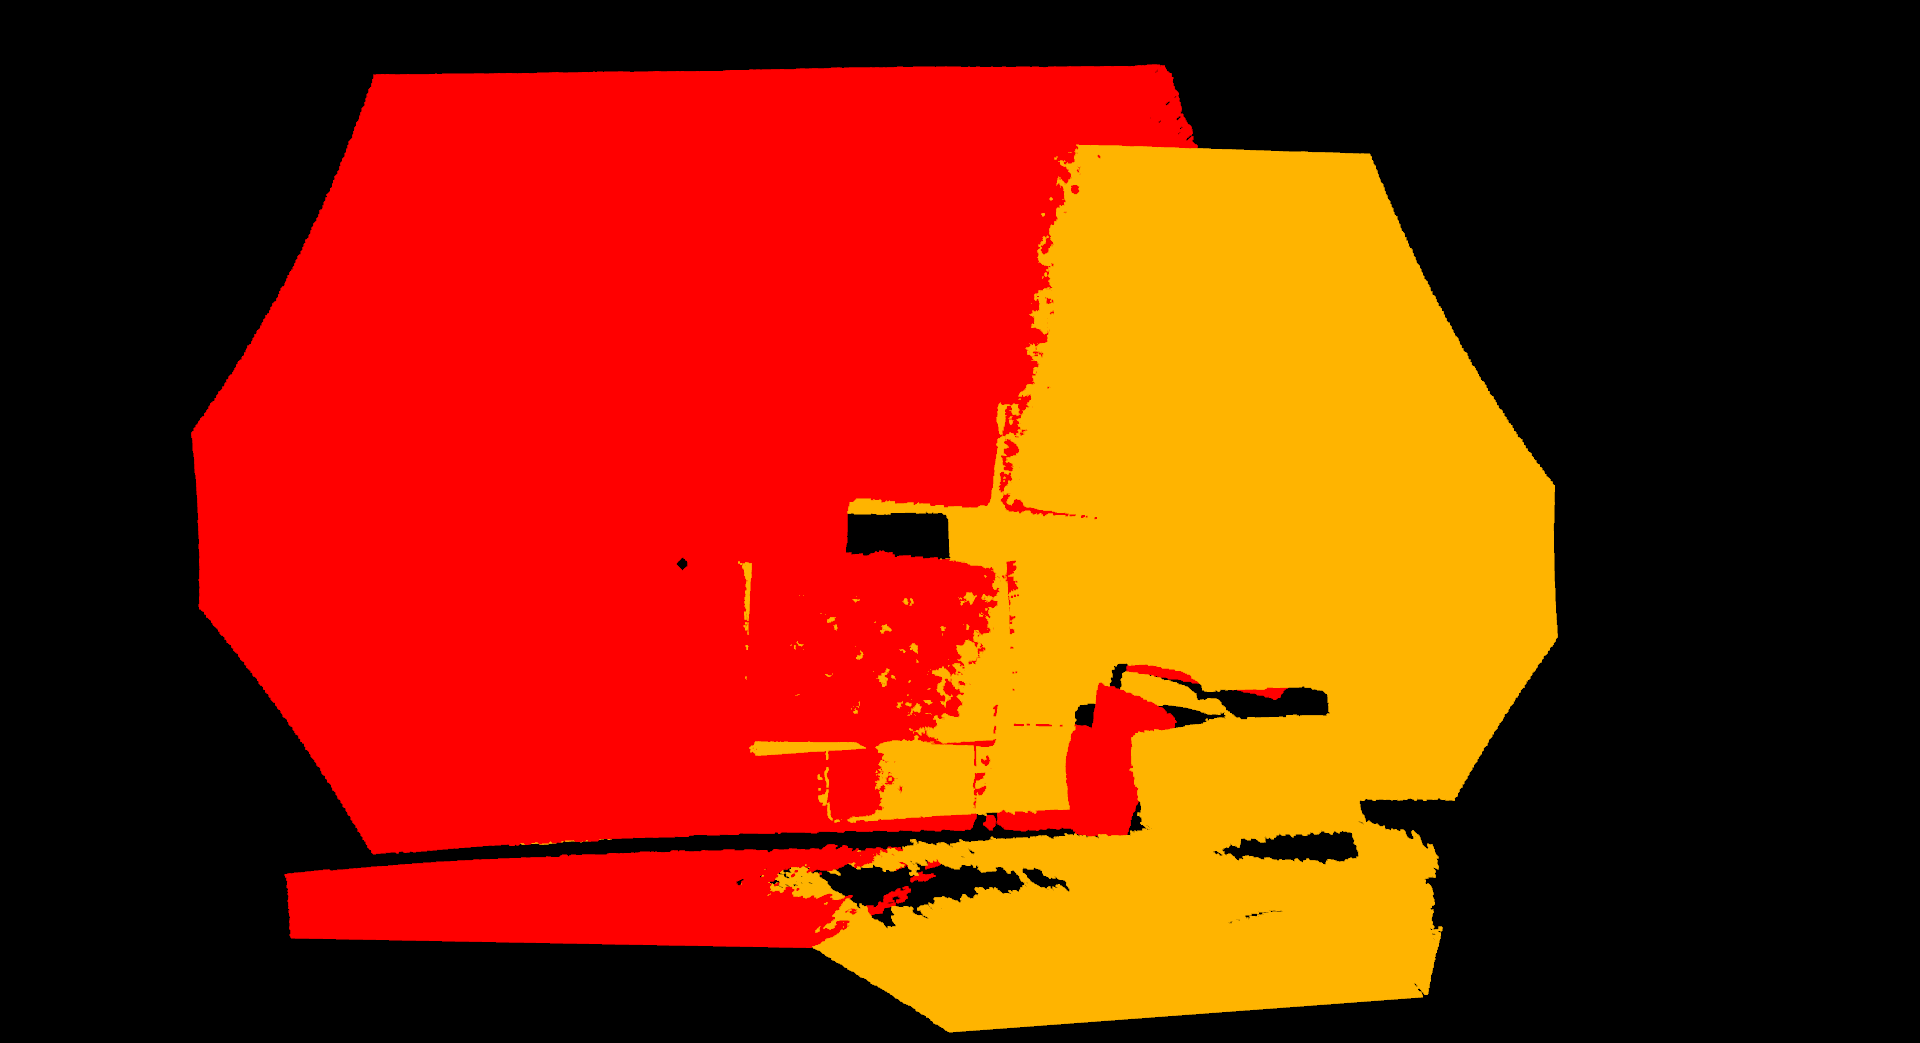
\includegraphics[width=\textwidth]{images/registration/init_ransac_colour.png}
    \caption{Alignment after the refine step}
    \label{figure:init_ransac_colour}
  \end{subfigure}
  \caption{Alignment of the two point clouds created from the two different views after the initialisation. The initialisation is made with a transformation matrix found by a RANSAC step. The point of view is virtual}
  \label{figure:init_ransac}
\end{figure}

Table \ref{tab:icp_1} shows the result of the different ICP methods. The colour registration method gives the best result. Taking into account the colour to find the transformation matrix helps the ICP algorithm. In opposite, point-to-point ICP doesn't improve the result of the initial step.

\begin{table}[H]
\begin{tabular}{c|c|c|c}
 & \textbf{X - coordinate} & \textbf{Y - coordinate} & \textbf{Z - coordinate} \\ \hline
\textbf{\begin{tabular}[c]{@{}c@{}}Mean Absolute Error\\ intial {[}mm{]}\end{tabular}} & 6.05 & 13.14 & 20.11 \\ \hline
\textbf{\begin{tabular}[c]{@{}c@{}}Mean Absolute Error\\ point-to-plane ICP {[}mm{]}\end{tabular}} & 6.87 & 9.56 & 15.03 \\ \hline
\textbf{\begin{tabular}[c]{@{}c@{}}Mean Absolute Error\\ point-to-point ICP {[}mm{]}\end{tabular}} & 7.51 & 14.58 & 19.12 \\ \hline
\textbf{\begin{tabular}[c]{@{}c@{}}Mean Absolute Error\\ coloured ICP {[}mm{]}\end{tabular}} & 2.17 & 2.67 & 2.51
\end{tabular}
\caption{Mean absolute error for the different ICP methods}
\label{tab:icp_1}
\end{table}

\textbf{Experiment 2}

For this experiment, the wall in the background is removed. Figure \ref{figure:init_ransac_crop} shows the initial situation before  launching the different ICP methods.

\begin{figure}[H]
\centering
  \begin{subfigure}[b]{0.48 \textwidth}
    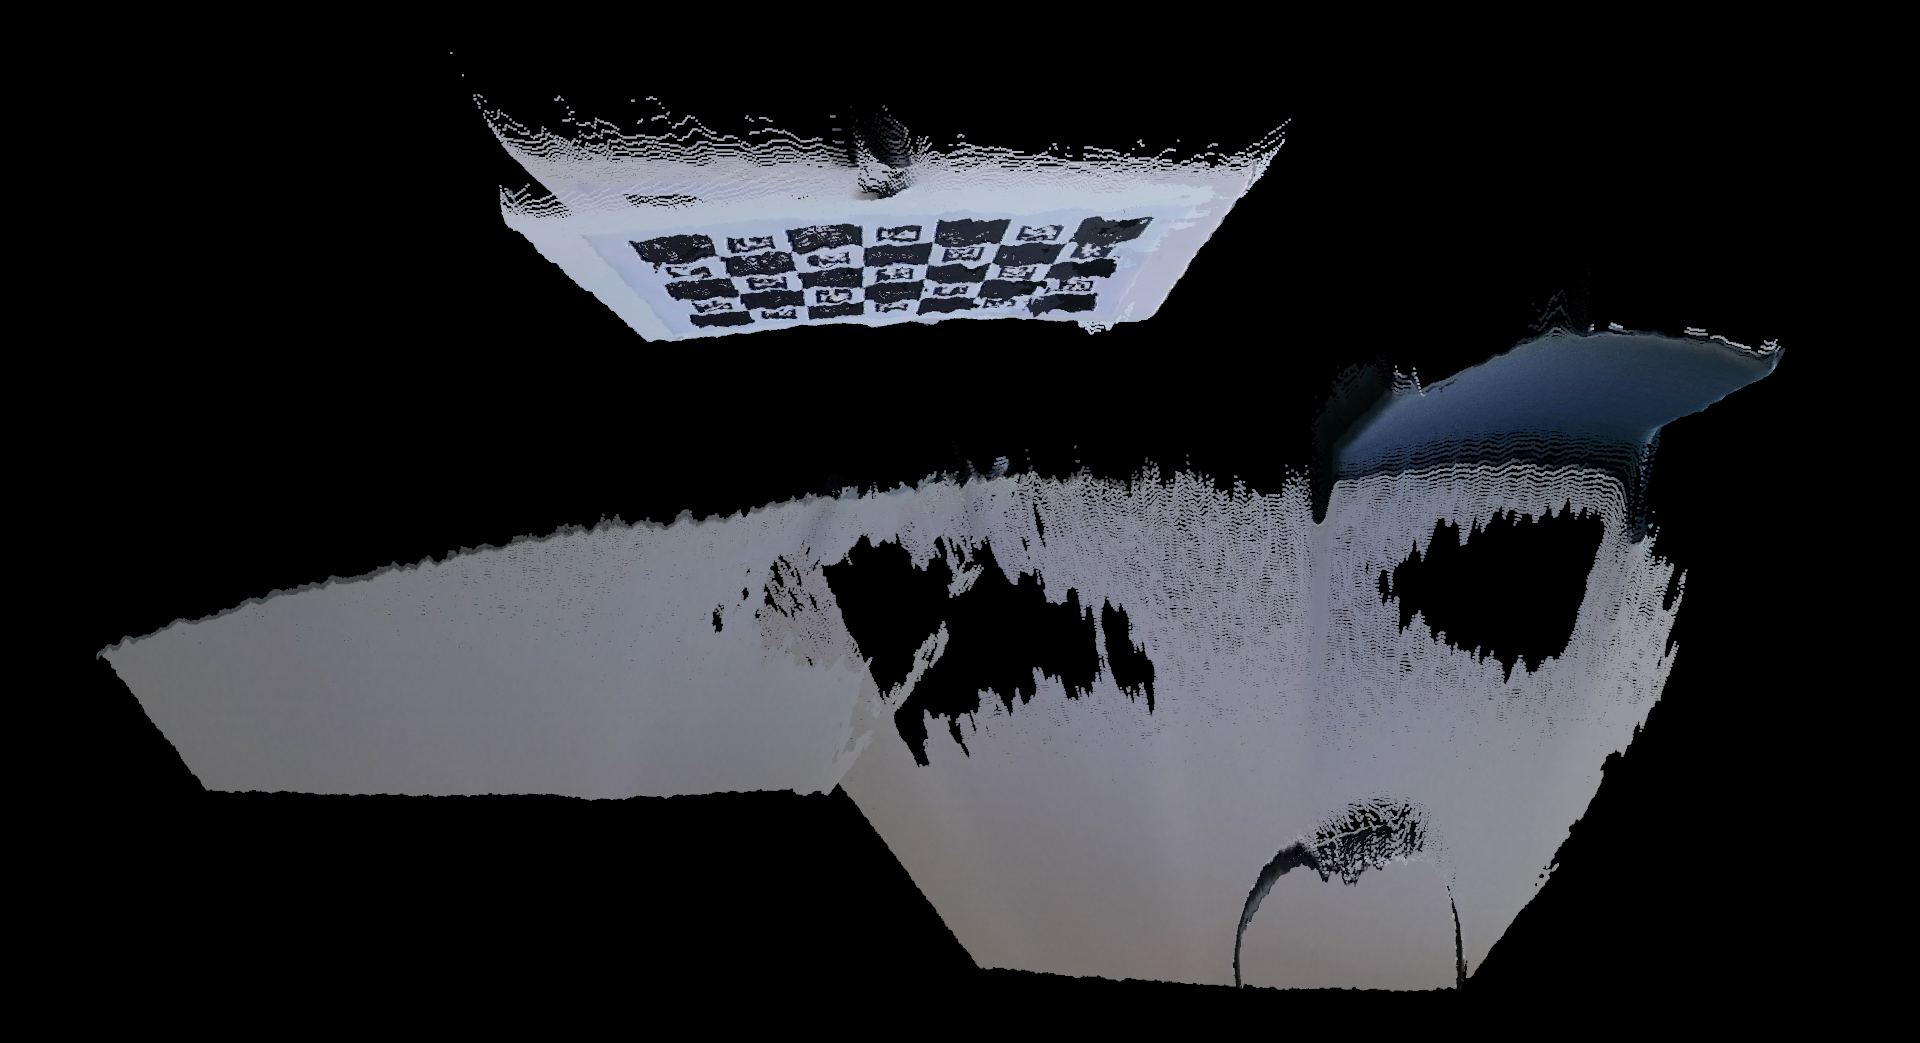
\includegraphics[width=\textwidth]{images/registration/init_ransac_crop_RGB.png}
    \caption{Alignment after the initialisationn}
    \label{figure:init_ransac_crop_RGB}
  \end{subfigure}
  \hfill
  \begin{subfigure}[b]{0.48 \textwidth}
    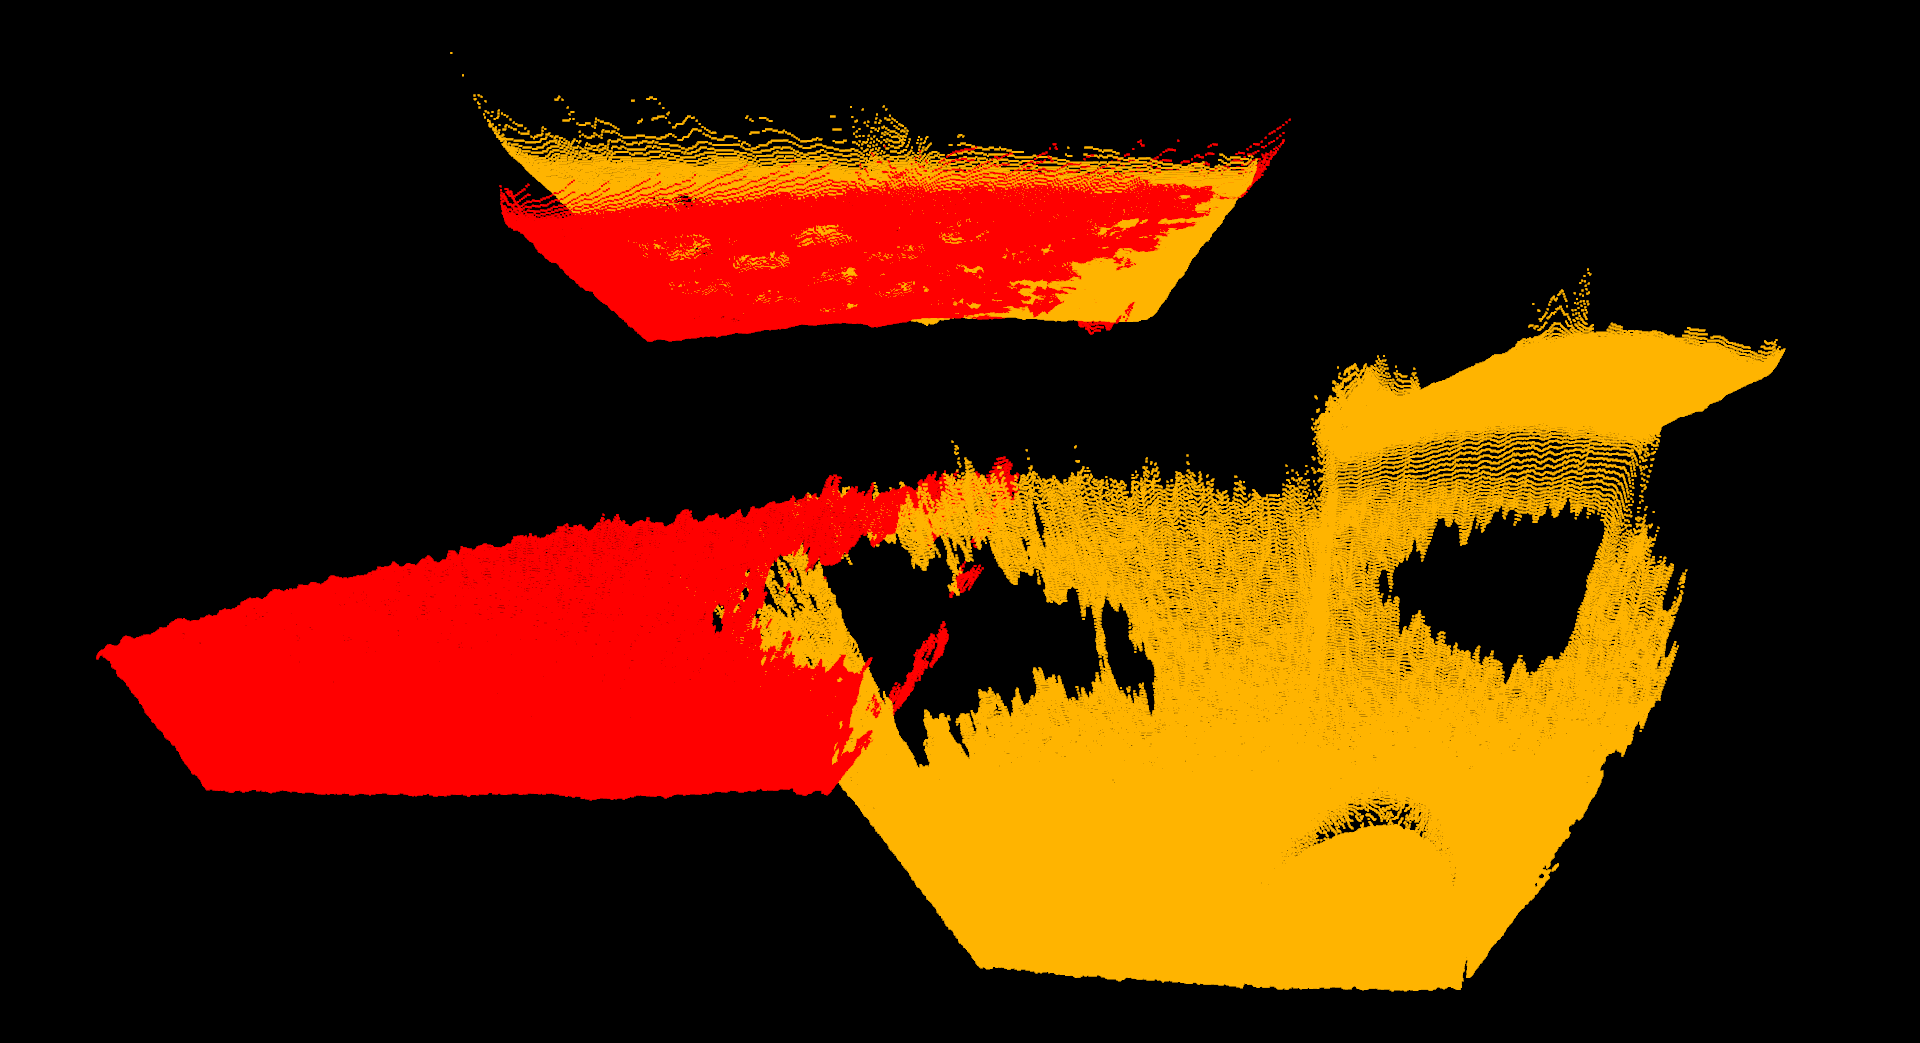
\includegraphics[width=\textwidth]{images/registration/init_ransac_crop_colour.png}
    \caption{Red: point cloud 1. Yellow: point cloud 2.}
    \label{figure:init_ransac_crop_colour}
  \end{subfigure}
  \caption{Alignment of the two point clouds created from the two different views after the initialisation. The initialisation is made with a transformation matrix found by a RANSAC step. The point of view is virtual.}
  \label{figure:init_ransac_crop}
\end{figure}

Table \ref{tab:icp_2} presents the result of the different ICP methods tried. The same observation as in experiment 1 can be made. Point-to-point ICP doesn't improve much the initial result. Coloured registration gives the best result. The colour information helps especially in the case of flat surfaces. 

\begin{table}[H]
\begin{tabular}{c|c|c|c}
 & \textbf{X - coordinate} & \textbf{Y - coordinate} & \textbf{Z - coordinate} \\ \hline
\textbf{\begin{tabular}[c]{@{}c@{}}Mean Absolute Error\\ intial {[}mm{]}\end{tabular}} & 6.05 & 13.14 & 20.11 \\ \hline
\textbf{\begin{tabular}[c]{@{}c@{}}Mean Absolute Error\\ point-to-plane ICP {[}mm{]}\end{tabular}} & 3.58 & 5.88 & 7.11 \\ \hline
\textbf{\begin{tabular}[c]{@{}c@{}}Mean Absolute Error\\ point-to-point ICP {[}mm{]}\end{tabular}} & 5.63 & 10.92 & 16.08 \\ \hline
\textbf{\begin{tabular}[c]{@{}c@{}}Mean Absolute Error\\ coloured ICP {[}mm{]}\end{tabular}} & 1.11 & 1.06 & 4.60
\end{tabular}
\caption{Mean absolute error for the different ICP methods}
\label{tab:icp_2}
\end{table}

\subsubsection{Stereo calibration}

For this experiment, the intrinsic parameters provided by the manufacturer of the Azure Kinect camera, i.e. Microsoft, are used to calibrate the camera. A chessboard is used as an easily detectable pattern. Corners position are recorded only if they are detected in both views. The OpenCV library \cite{noauthor_opencv_nodate} is used to detect the corners in an image. According to the documentation, a better estimation of the extrinsic parameters is obtained if several images are recorded in different positions and orientations. For the purpose of this experiment, fifty images are taken. Figure \ref{figure:corner} shows a sample of the used images.

\begin{figure}[H]
\centering
  \begin{subfigure}[b]{0.48 \textwidth}
    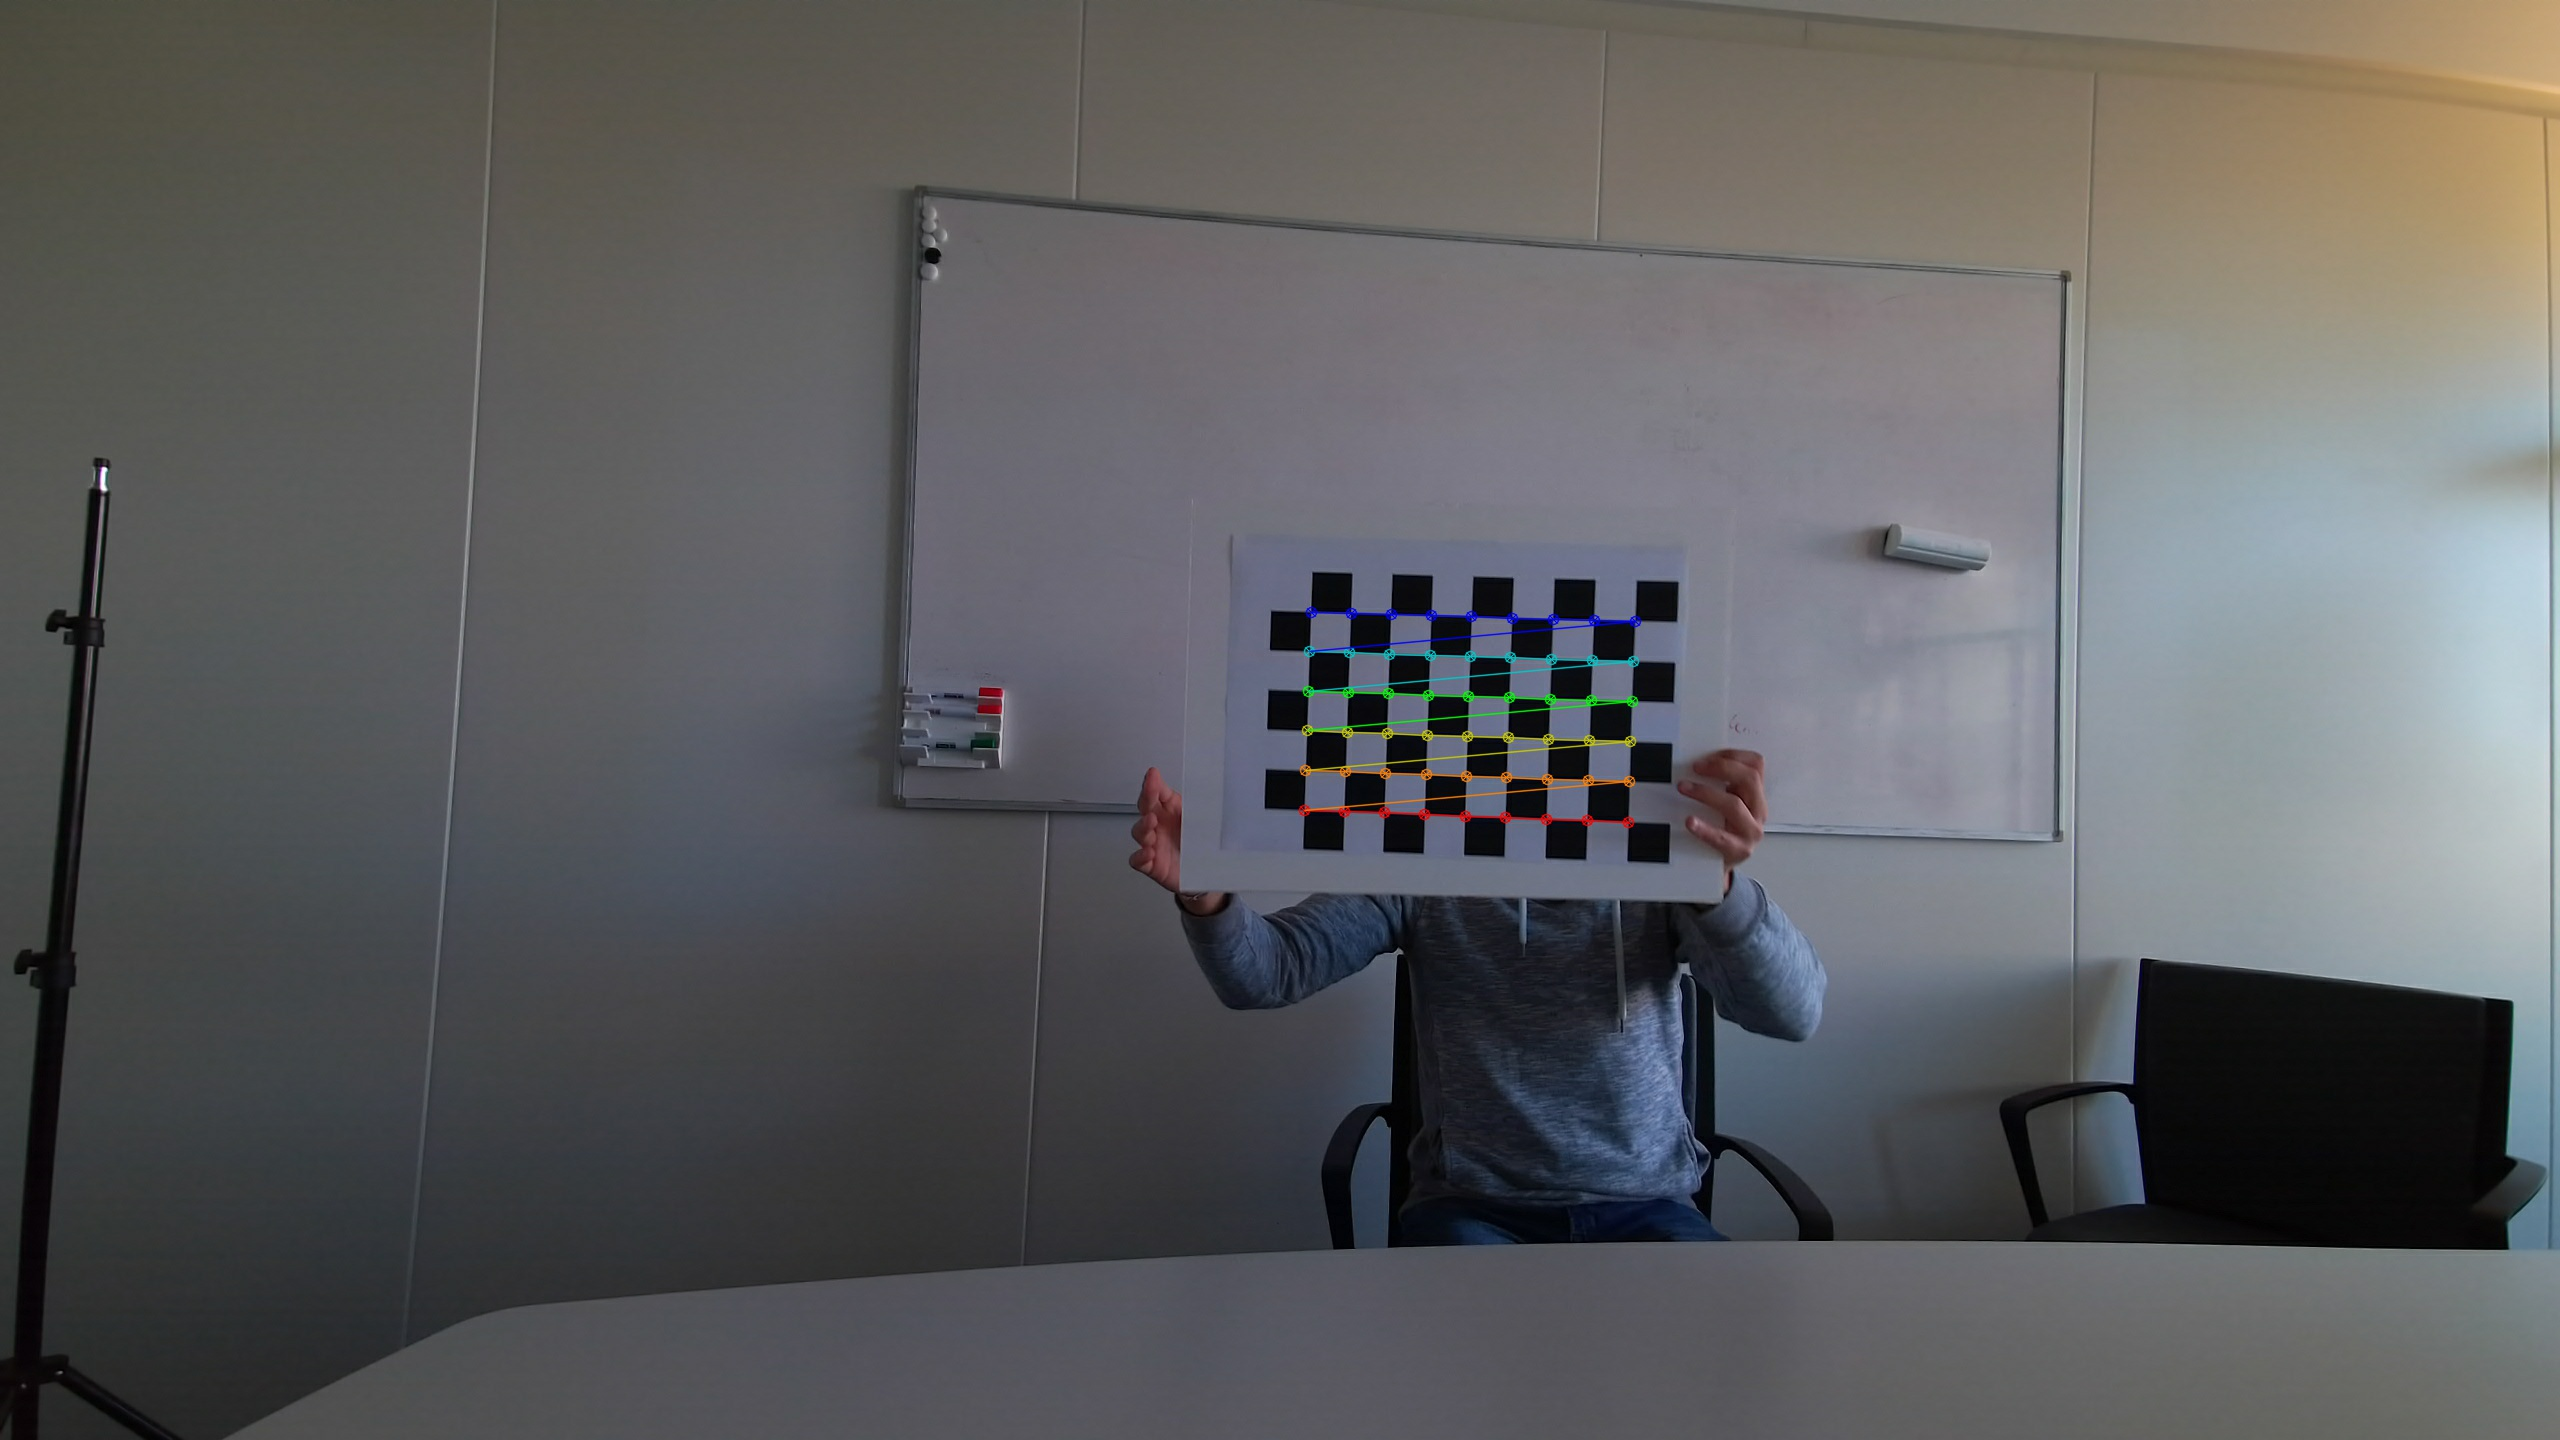
\includegraphics[width=\textwidth]{images/registration/corner_sub_4.jpg}
    \caption{Chessboard viewed from camera 1}
    \label{figure:corner_sub_4}
  \end{subfigure}
  \hfill
  \begin{subfigure}[b]{0.48\textwidth}
    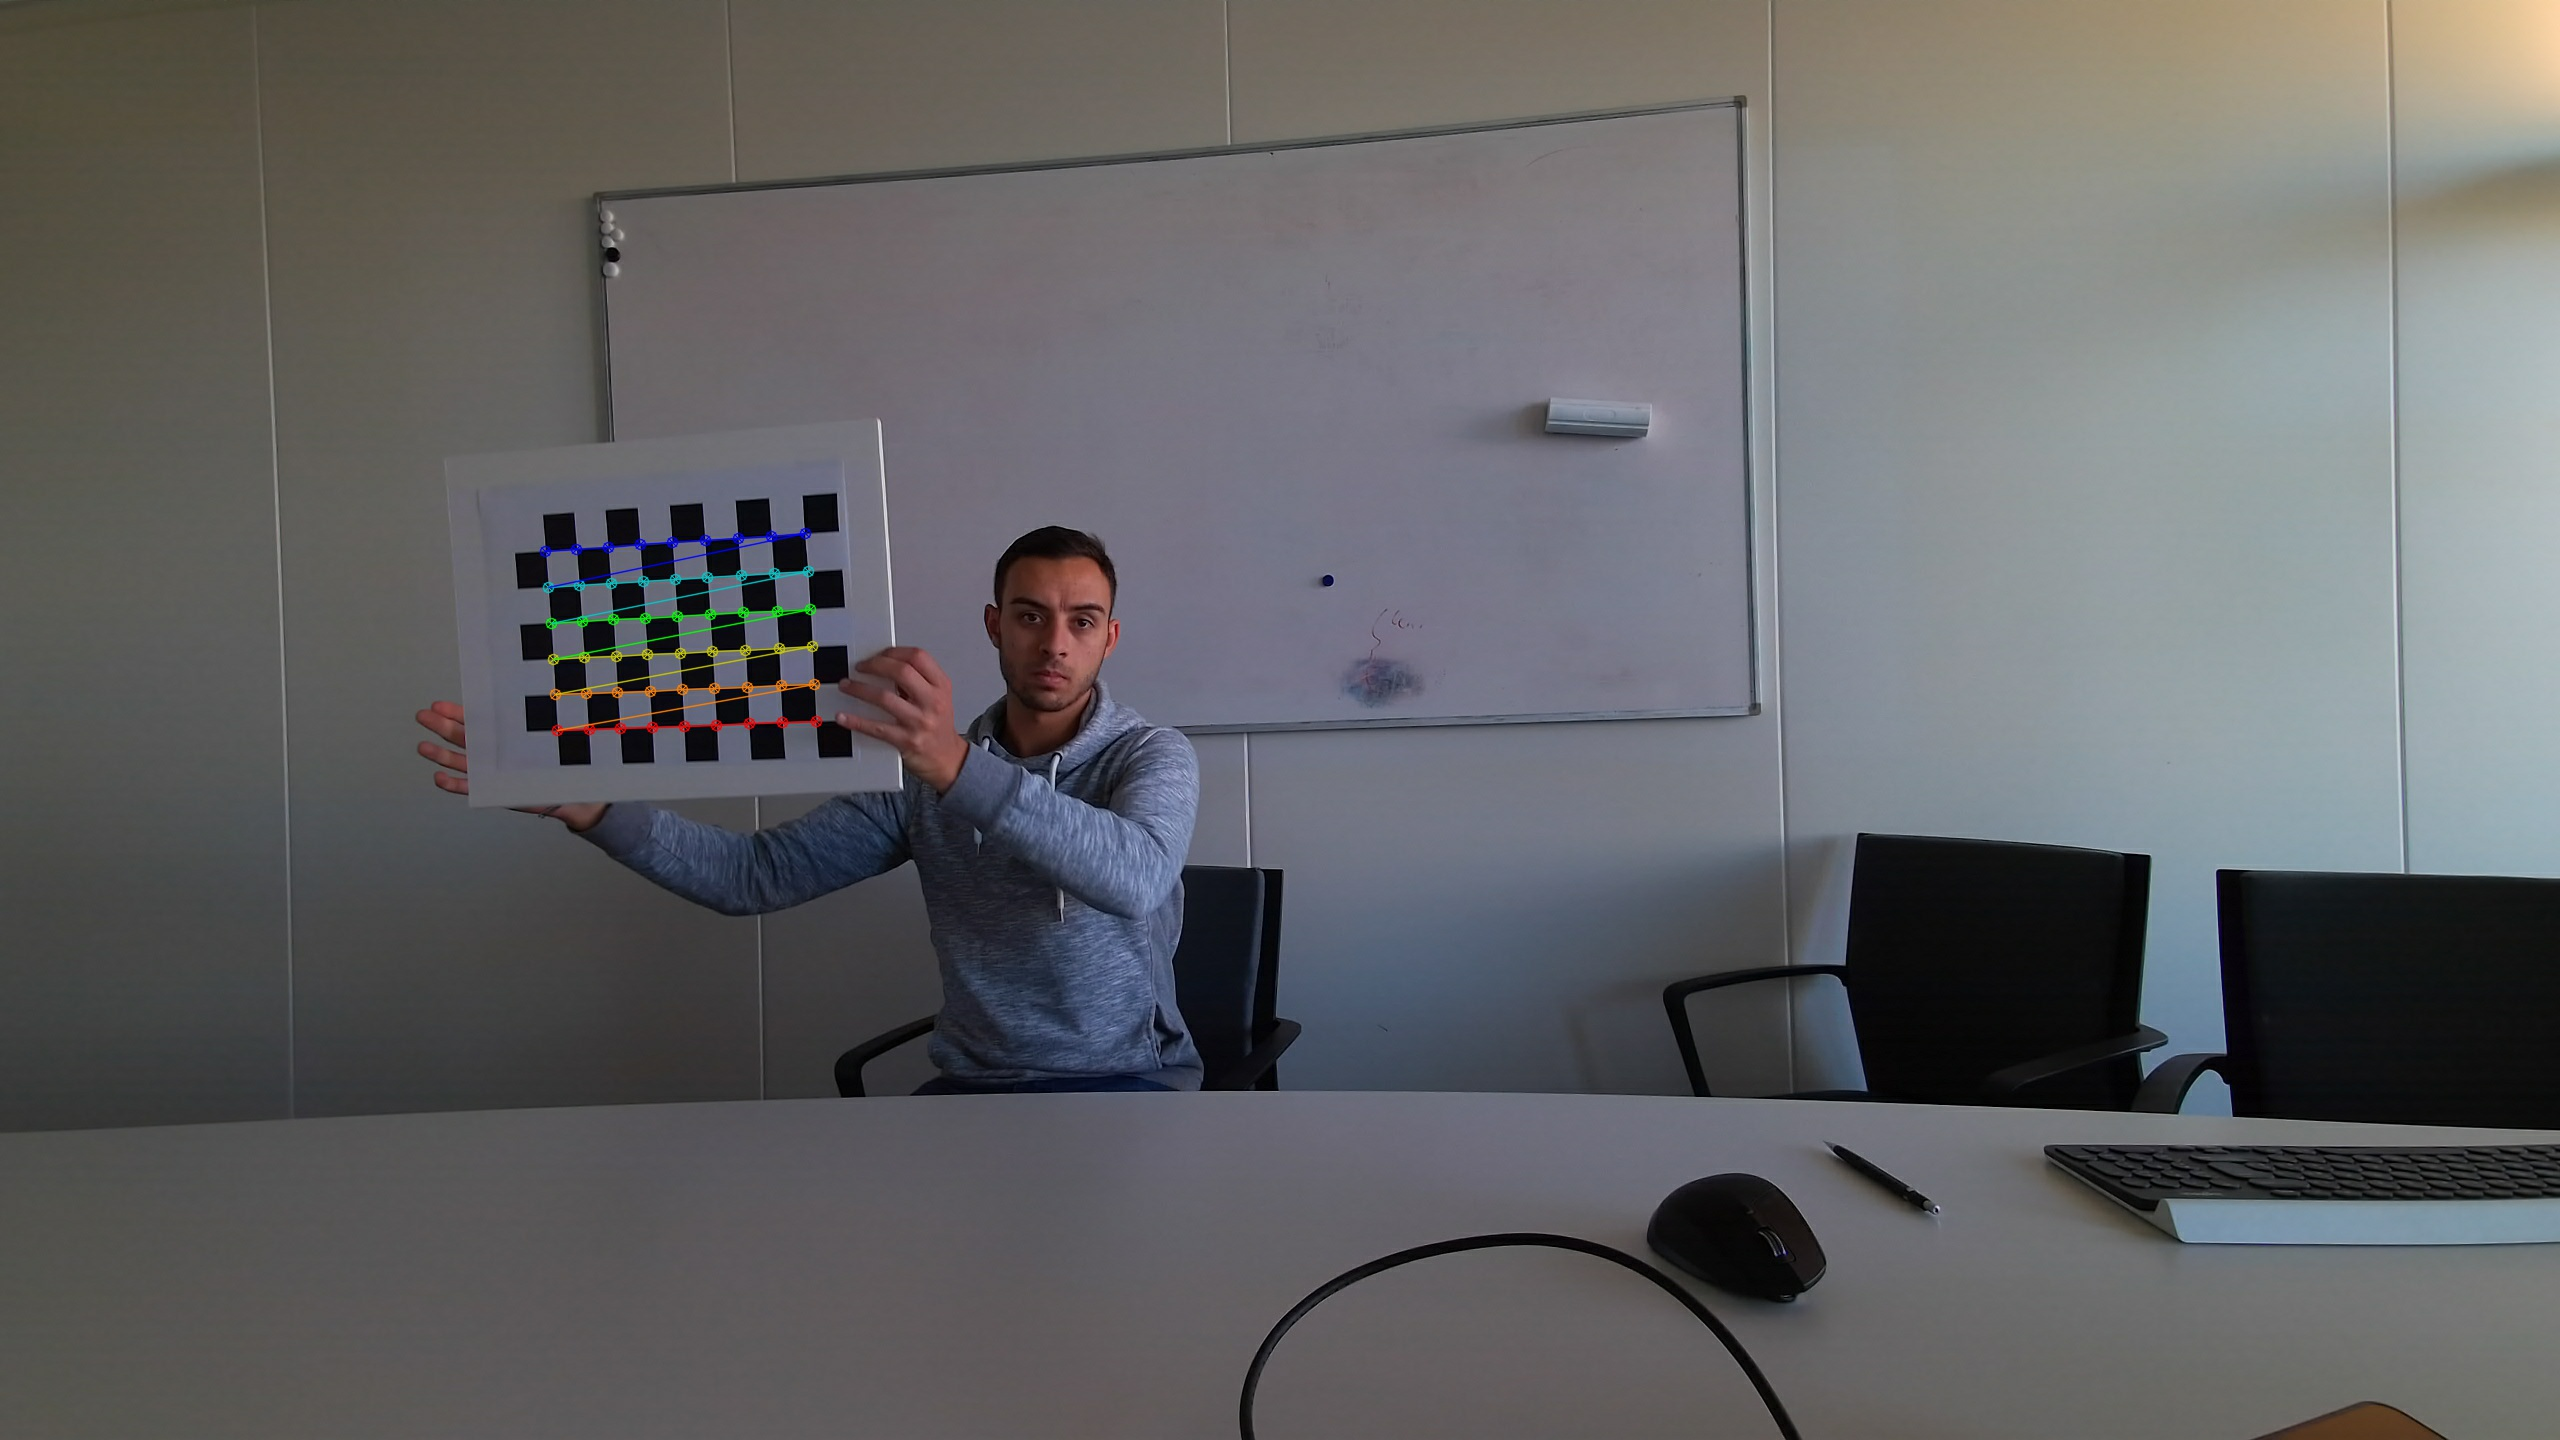
\includegraphics[width=\textwidth]{images/registration/corner_master_4.jpg}
    \caption{Chessboard viewed from camera 2}
    \label{figure:corner_master_4}
  \end{subfigure}
  \caption{Detection of the chessboard corners viewed from both cameras at the same time}
  \label{figure:corner}
\end{figure}

The function \textit{StereoCalibrate} provided by OpenCV is then used. It estimates transformation between two cameras making a stereo pair. One of the outputs is the estimation of the transformation matrix between the coordinate systems of the first and the second cameras.

% \todo{is this figure relevant?}
% \begin{figure}[H]
%     \centering
%     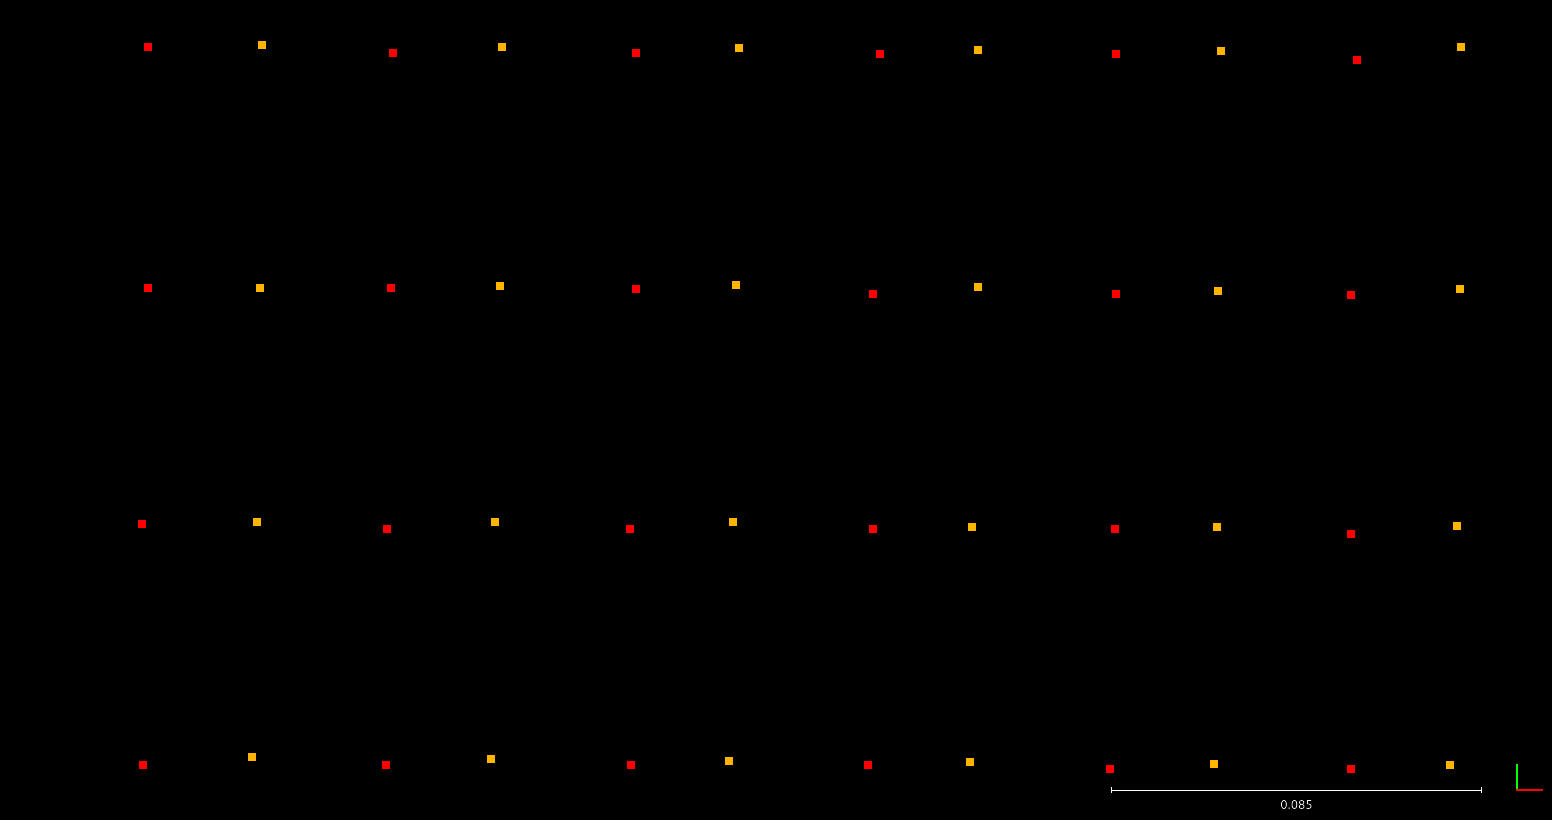
\includegraphics[width=0.65\textwidth]{images/registration/chessboard_transfo.png}
%     \caption{Plan XY. Red points: ChArUco board point cloud from the 1st camera. Yellow points: ChArUco board point cloud from the 2nd camera. Scale is in meter}
%     \label{figure:chessboard_transfo}
% \end{figure}

Table \ref{tab:mae_chessboard} presents the results after applying the found transformation matrix on one of the ChArUco point clouds of figure \ref{figure:pc_arucoboard}. The error in the X-coordinate is quite big, see table \ref{tab:mae_chessboard}. This results in a noticeable misalignment when applied on live sequence with a person in it. Figure \ref{figure:stereo_misaligned} shows a selected frame where the misalignment is visible.

\begin{table}[H]
\centering
\begin{tabular}{c|c|c|c}
 & \textbf{X - coordinate} & \textbf{Y - coordinate} & \textbf{Z - coordinate} \\ \hline
\textbf{Mean Absolute Error {[}mm{]}} & 24.07 & 1.09 & 4.54
\end{tabular}
\caption{Mean absolute error for the stereo calibration experiment with the chessboard}
\label{tab:mae_chessboard}
\end{table}

\begin{figure}[H]
\centering
  \begin{subfigure}[b]{0.48 \textwidth}
    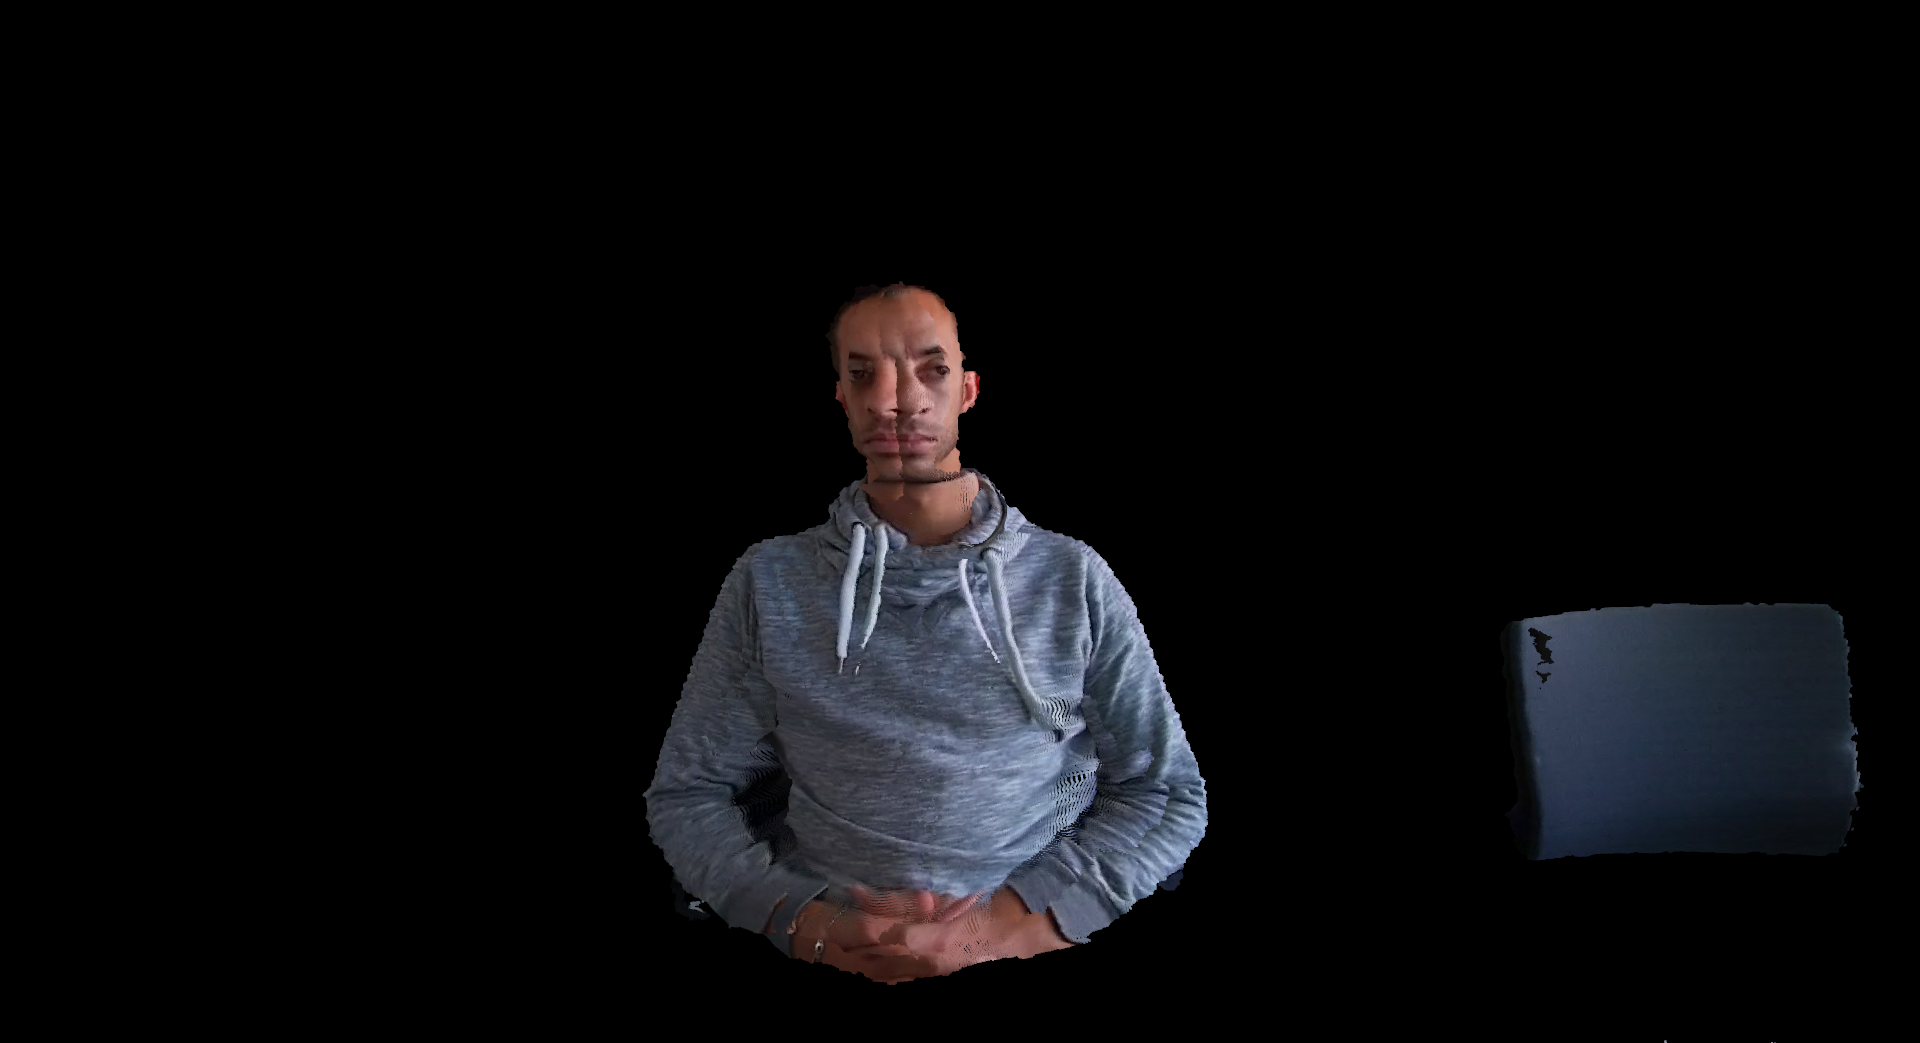
\includegraphics[width=\textwidth]{images/registration/stereo_RGB.png}
    \caption{Alignment after applying the found matrix}
    \label{figure:stereo_RGB}
  \end{subfigure}
  \hfill
  \begin{subfigure}[b]{0.48\textwidth}
    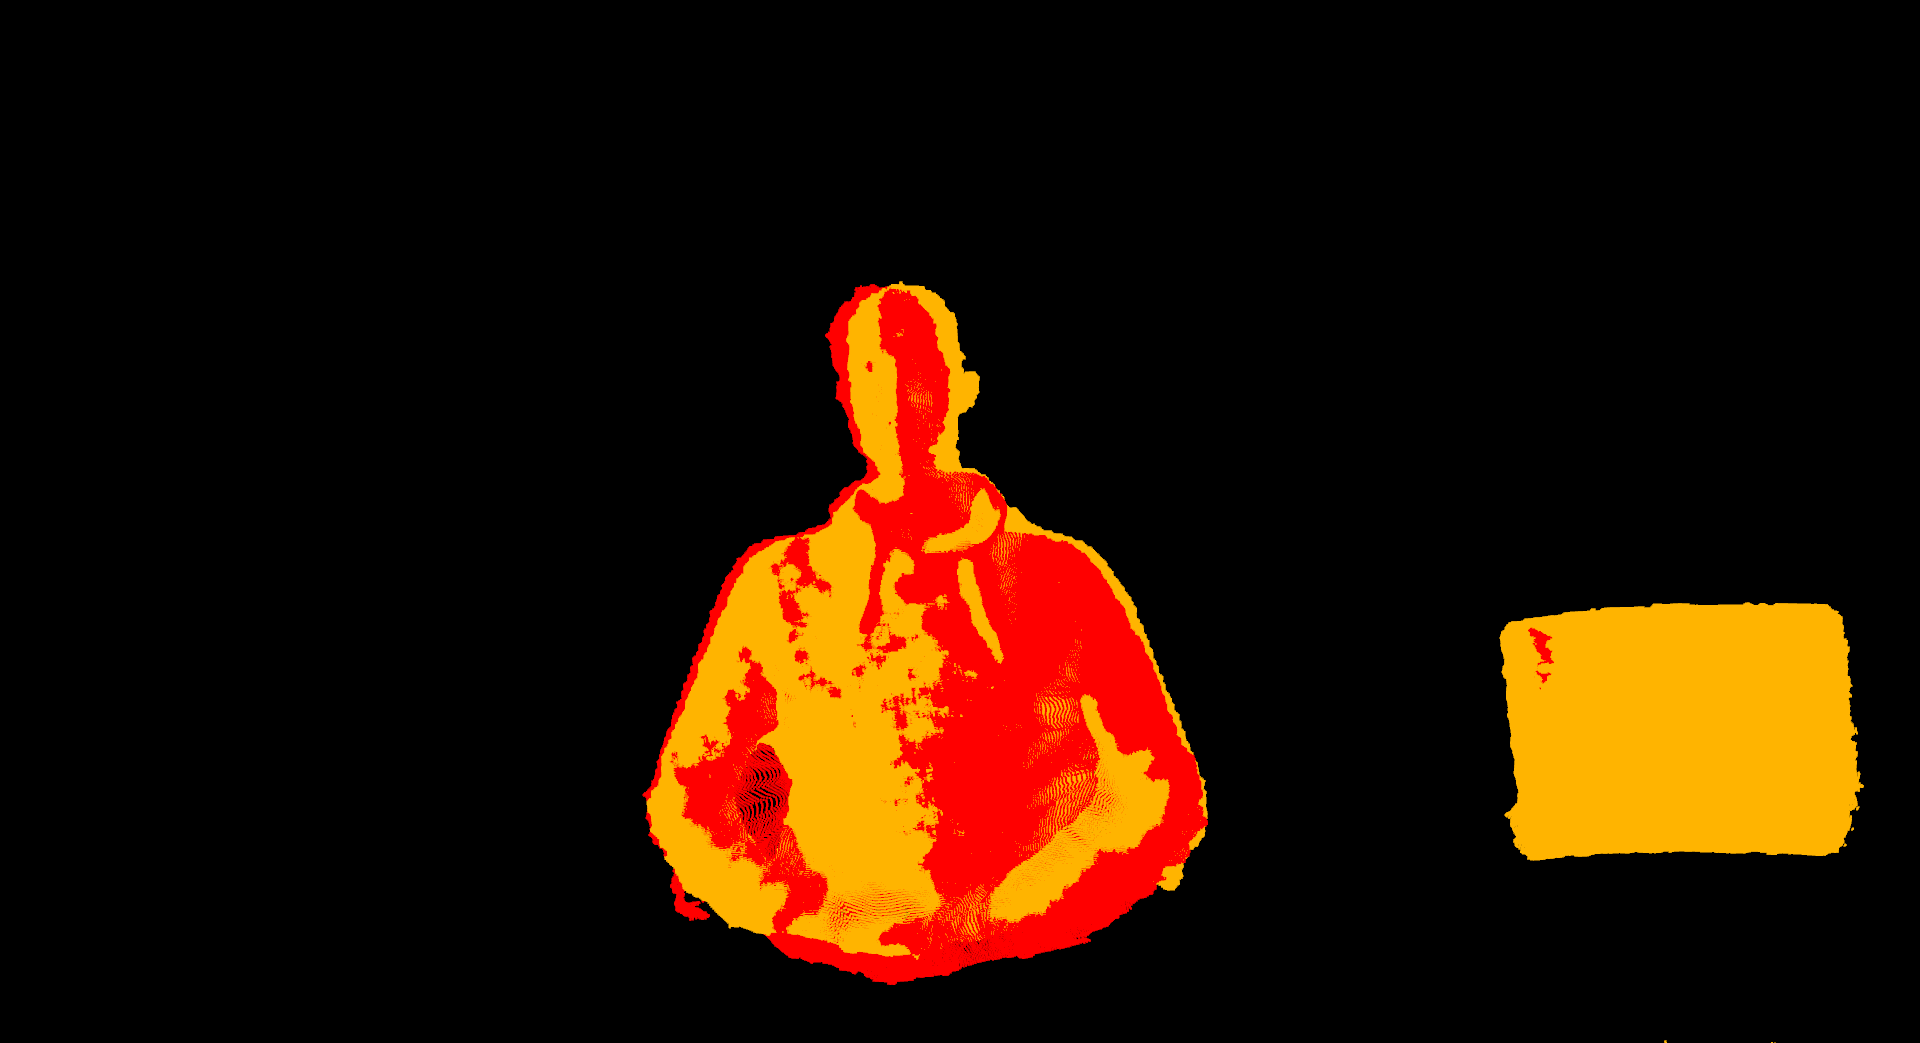
\includegraphics[width=\textwidth]{images/registration/stereo_colored.png}
    \caption{Red: point cloud 1. Yellow: point cloud 2}
    \label{figure:stereo_colored}
  \end{subfigure}
  \caption{Alignment of the two point clouds created from the two different views after applying the transformation matrix found by stereo calibration}
  \label{figure:stereo_misaligned}
\end{figure}

\subsubsection{Proposed method}

The approach explained in section \ref{section:proposed_method} is applied to this experiment. A ChArUco board is placed in the centre of the scene. 100 frames are taken in a synchronised way from both views. The pixel positions of the corners are extracted with their corresponding depth and averaged over the frames. Then two point clouds are created, i.e. one per camera, with the help of equation (\ref{equation:2dTO3d}). Finally, a function provided by Open3D \cite{Zhou2018} is used.

\begin{table}[H]
\begin{tabular}{c|c|c|c}
 & \textbf{X - coordinate} & \textbf{Y - coordinate} & \textbf{Z - coordinate} \\ \hline
\textbf{Mean Absolute Error (MAE) {[}mm{]}} & 0.90 & 0.48 & 0.40
\end{tabular}
\caption{Mean absolute error for the stereo calibration experiment of the proposed method}
\label{tab:mae_proposed_method}
\end{table}

Table \ref{tab:mae_proposed_method} presents the different MAE. As this error is below 1 mm, it is barely visible in a dynamic scene. Figure \ref{figure:proposed_method_alignment} shows a selected frame.

% One can notice the misalignment only when the zoom is quite high, see figure ...

\begin{figure}[H]
\centering
  \begin{subfigure}[b]{0.48 \textwidth}
    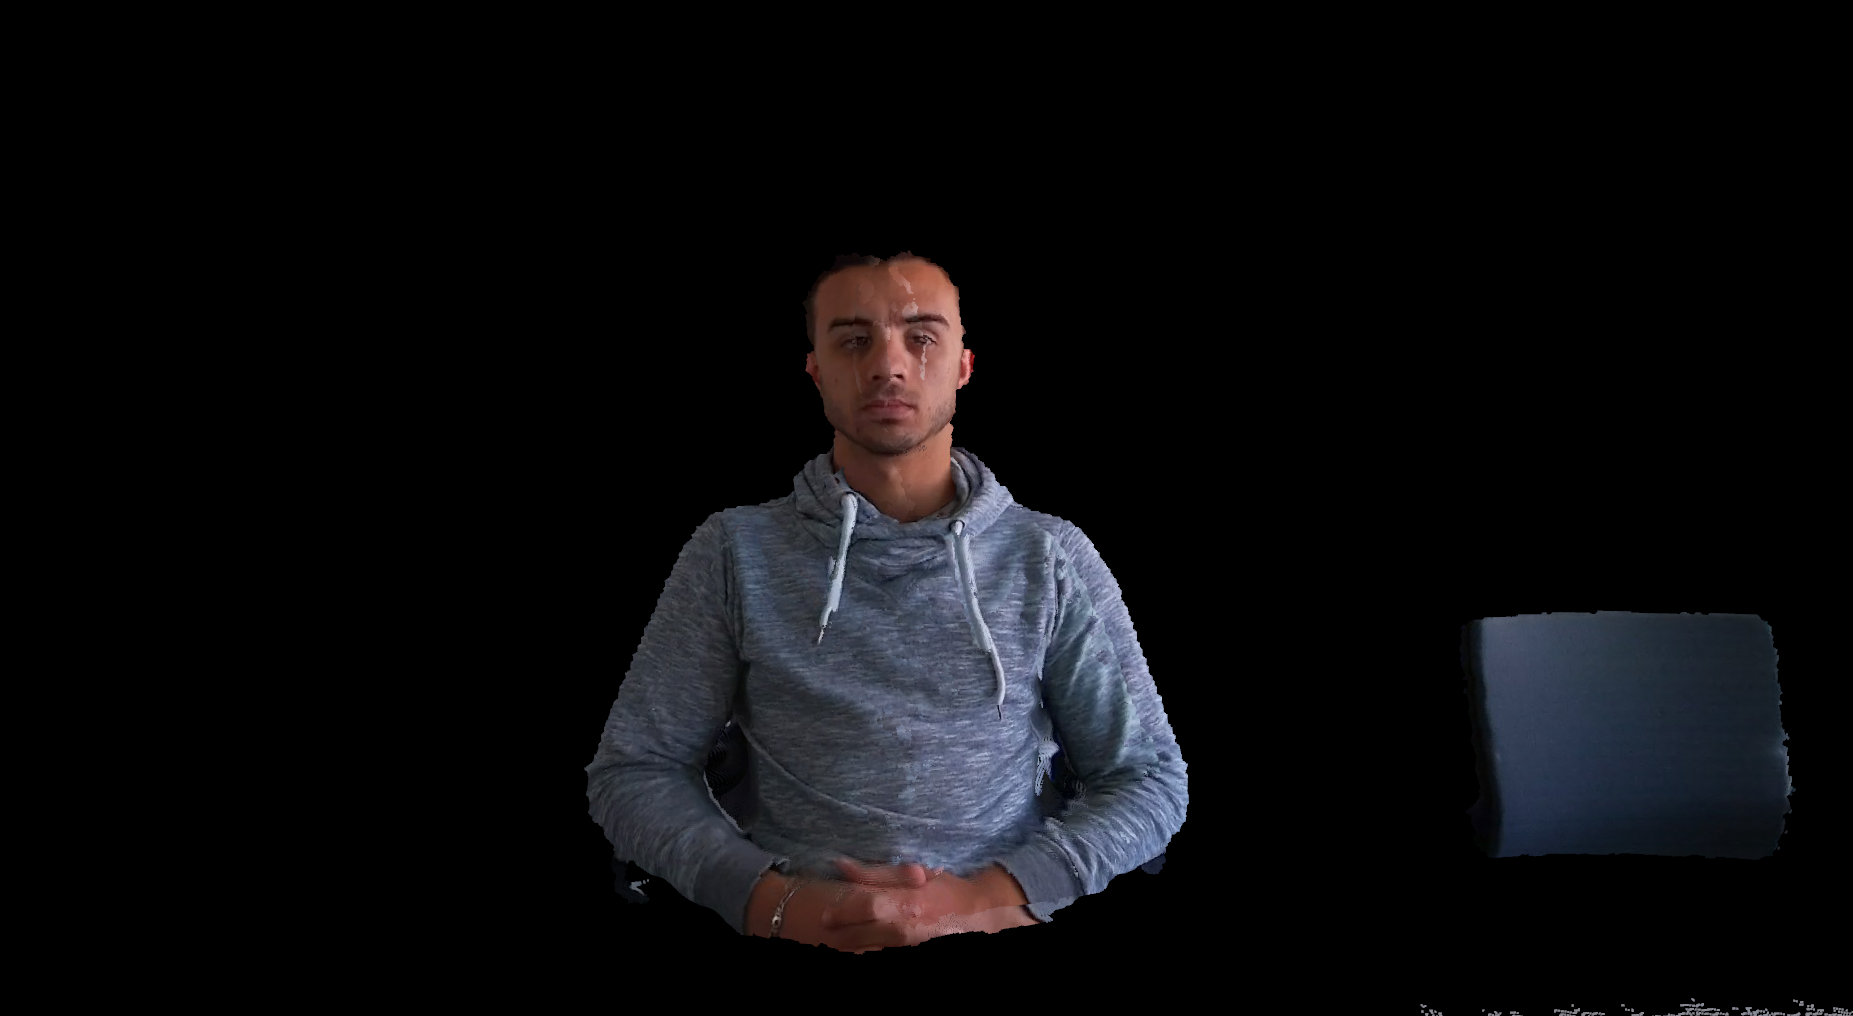
\includegraphics[width=\textwidth]{images/registration/proposed_method_RGB.png}
    \caption{Alignment after applying the found matrix}
    \label{figure:stereo_RGB}
  \end{subfigure}
  \hfill
  \begin{subfigure}[b]{0.48\textwidth}
    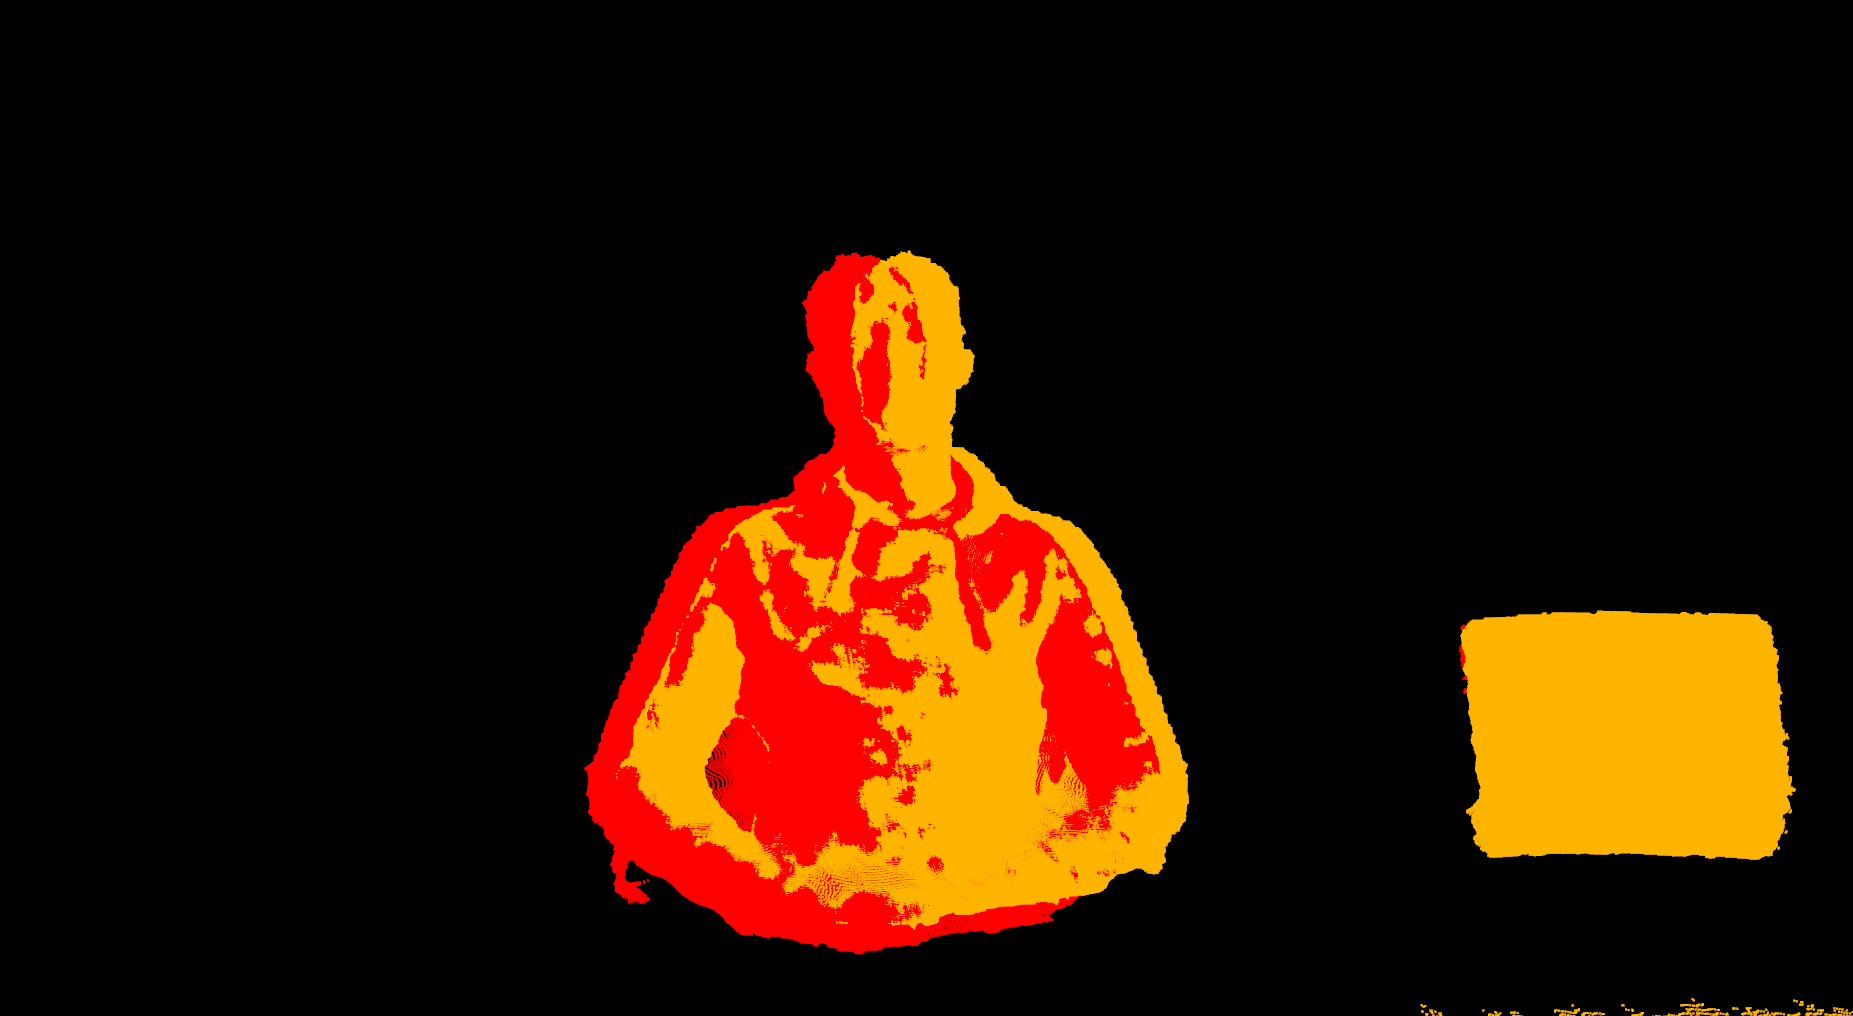
\includegraphics[width=\textwidth]{images/registration/proposed_method_colour.png}
    \caption{Red: point cloud 1. Yellow: point cloud 2}
    \label{figure:stereo_colored}
  \end{subfigure}
  \caption{Alignment of the two point clouds created from the two different views after applying the transformation matrix found by the proposed method}
  \label{figure:proposed_method_alignment}
\end{figure}



Despite a good alignment in the region around the ChArUco board, a small misalignment is visible in the background for example, see figure \ref{figure:proposed_method_background}. One reason could come from the intrinsic parameters. They are used to create the point clouds. So if they are not exact, it could create a slightly deformed point cloud. Another reason  could come from the fact that the background is further away from the board. So even if this error is small on the region around the board, this error becomes more noticeable outside the calibrated region.

\begin{figure}[H]
    \centering
    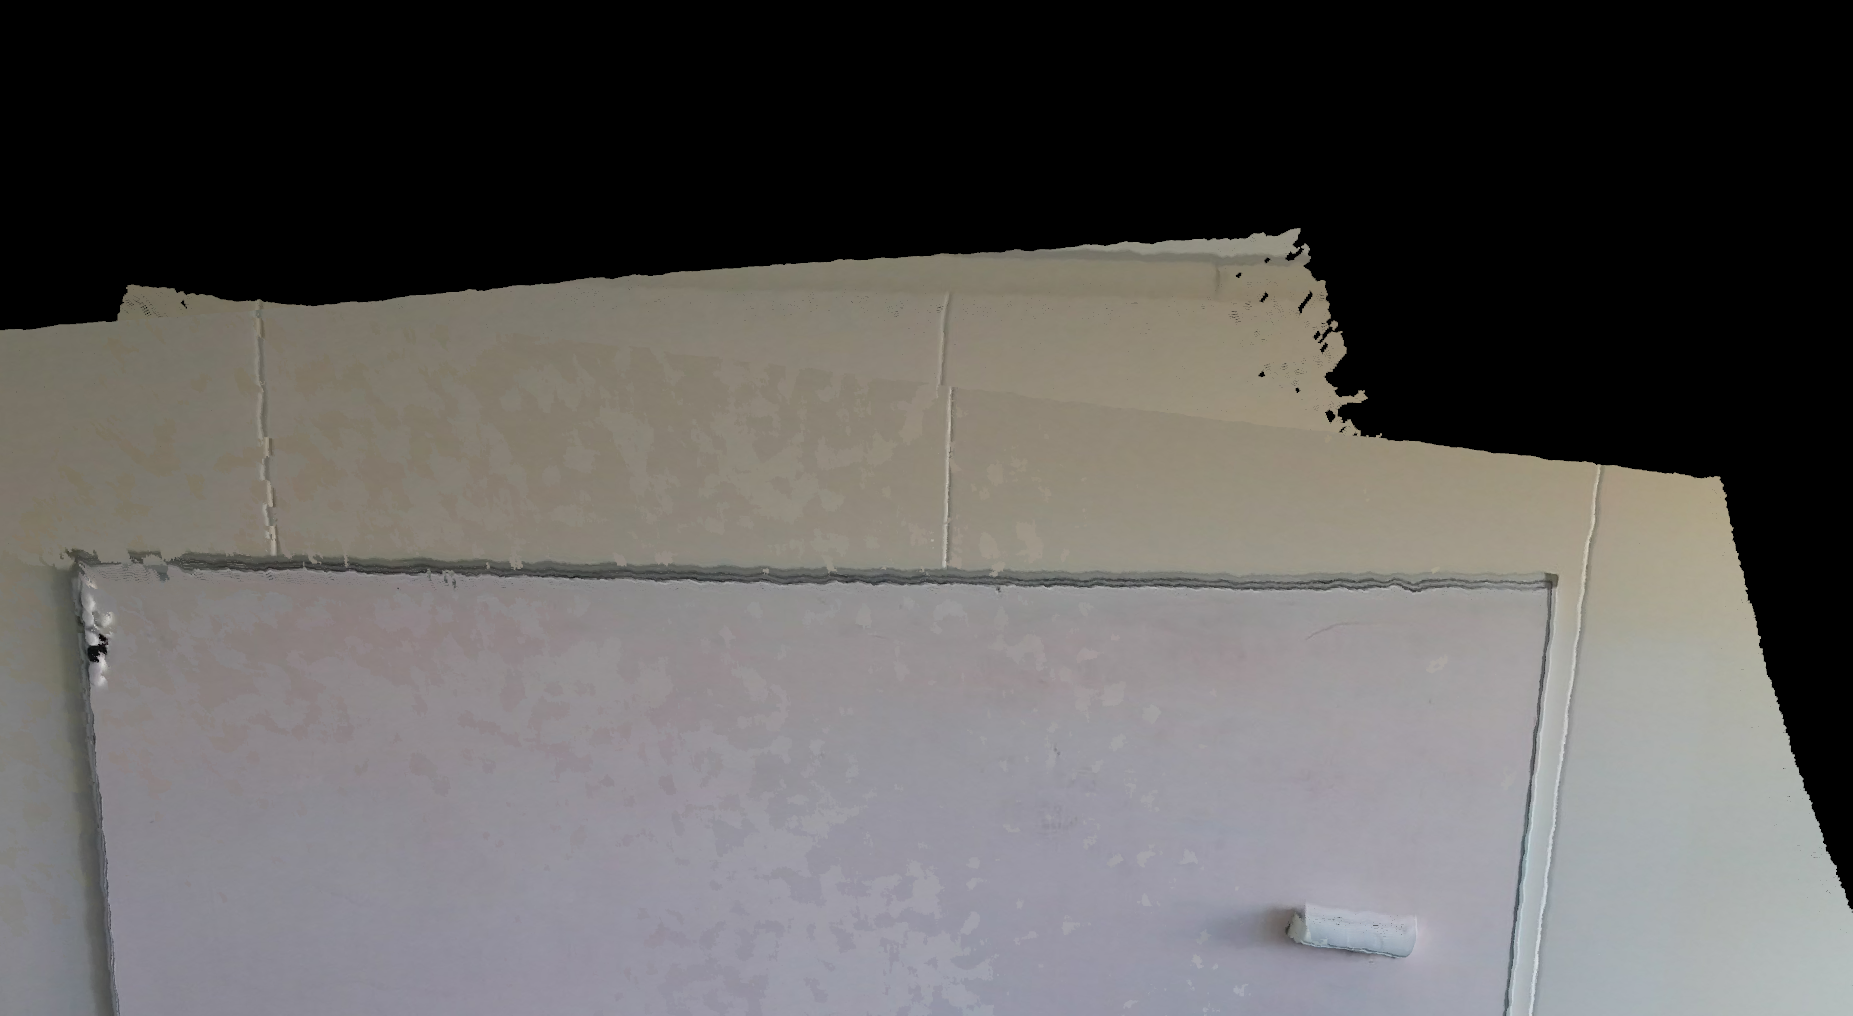
\includegraphics[width=0.65\textwidth]{images/registration/proposed_method_background.png}
    \caption{Small misalignment in the background}
    \label{figure:proposed_method_background}
\end{figure}

\subsection{General Result}

Table \ref{tab:sumary_registration} presents the summary of the results of the different approaches developed in the previous sections. The proposed method gives the best result.


\begin{table}[H]
\centering
\begin{tabular}{c||c|c|c}
\textbf{Mean Absolute Error of} & \textbf{X - coordinate} & \textbf{Y - coordinate} & \textbf{Z - coordinate} \\ \hline \hline
\textbf{\begin{tabular}[c]{@{}c@{}}Global registration\\ Experiment 2 {[}mm{]}\end{tabular}} & 3.04 & 0.57 & 2.40 \\ \hline
\textbf{\begin{tabular}[c]{@{}c@{}}Global registration\\ Experiment 3 {[}mm{]}\end{tabular}} & 13.81 & 1.29 & 1.33 \\ \hline \hline
\textbf{\begin{tabular}[c]{@{}c@{}}Point-to-plane ICP\\ Experiment 1 {[}mm{]}\end{tabular}} & 6.87 & 9.56 & 15.03 \\ \hline
\textbf{\begin{tabular}[c]{@{}c@{}}Point-to-plane ICP\\ Experiment 2 {[}mm{]}\end{tabular}} & 3.58 & 5.88 & 7.11 \\ \hline \hline
\textbf{\begin{tabular}[c]{@{}c@{}}Point-to-point ICP\\ Experiment 1 {[}mm{]}\end{tabular}} & 7.51 & 14.58 & 19.12 \\ \hline
\textbf{\begin{tabular}[c]{@{}c@{}}Point-to-point ICP\\ Experiment 2 {[}mm{]}\end{tabular}} & 5.63 & 10.92 & 16.08 \\ \hline \hline
\textbf{\begin{tabular}[c]{@{}c@{}}Coloured ICP\\ Experiment 1 {[}mm{]}\end{tabular}} & 2.17 & 2.67 & 2.51 \\ \hline
\textbf{\begin{tabular}[c]{@{}c@{}}Coloured ICP\\ Experiment 2 {[}mm{]}\end{tabular}} & 1.11 & 1.06 & 4.60 \\ \hline \hline
\textbf{\begin{tabular}[c]{@{}c@{}}Stereo\\ calibration\end{tabular}} & 24.07 & 1.09 & 4.54 \\ \hline \hline
\textbf{\begin{tabular}[c]{@{}c@{}}Proposed\\ method\end{tabular}} & \textbf{0.90} & \textbf{0.48} & \textbf{0.40}
\end{tabular}
\caption{Summary of the mean absolute error of all the evaluated methods}
\label{tab:sumary_registration}
\end{table}


\subsection{Discussion}

The results of the ICP based approaches depend on the initialisation. This is a disadvantage because estimating the transformation is not straightforward. Even if the initialisation is close to the ideal transformation, these approaches are sensitive to the geometry of the scenes to align. This is also a disadvantage if the scene does not have the good characteristic. However, in case of an ideal scene, these approaches give good results. Coloured ICP helps in the case of flat surfaces. Using the colour of the scene for the alignment of a flat scene provides better results than the point-to-plane ICP and point-to-point ICP.

The global registration procedure is sensible to the geometry of the scene. The different experiments of the section \ref{section:Global registration result} demonstrate that variation in the geometry of the scene helps the RANSAC step finding corresponding points. In the case of a flat scene, the FPFH features are too similar. Therefore, finding relevant corresponding points is not successful. This approach is not robust. However, once the RANSAC step succeeds, the local refinement step depends then on the ICP performances. Point-to-plane ICP was used in these experiments and gave acceptable results. The other variation of ICP could have been applied as well.

The stereo calibration approach is not a success in the presented experiment. Several trials were made. The one presented is the one that gives the best results. The misalignment especially in the X-coordinate could probably be explained by the nature of the image taken to calculate the estimation of the transformation matrix. However, such a method depends on the image taken during the calibration process. It is a non-robust method.

The proposed method is the one that gives the best result, see table \ref{tab:sumary_registration}. The error is below 1 mm in the three different directions. This error is barely visible in a streaming application. Once the ChArUco board point clouds are created, the calculation of the transformation gives always the same result. This is  therefore a robust. 
A drawback is the fact that it is a local approach. It means that the resulting transformation gives good result in the region around the board but further away a misalignment could be noticeable. This method is the one chosen for all the next experiments and steps of this project. 

